\documentclass[UTF8,a4paper,zihao=-4]{ctexart}

\usepackage[left=2.55cm,right=2.45cm,top=2.45cm,bottom=2.45cm]{geometry}
\usepackage{amsmath,amssymb,bm}
\usepackage{booktabs,longtable,tabularx,array,multirow}
\usepackage{graphicx,float,caption,subcaption}
\usepackage{xcolor,fancyhdr,setspace,enumitem,placeins,hyperref}
\usepackage{listings}

\setmainfont{Times New Roman}
\setmonofont{Cascadia Mono}
\setCJKmainfont[AutoFakeBold=2]{SimSun}
\setCJKsansfont{Microsoft YaHei}
\setlength{\parindent}{2em}
\setlength{\parskip}{0pt}
\linespread{1.25}
\setlist{nosep,leftmargin=2.2em}
\captionsetup{font=small,labelsep=quad}
\graphicspath{{../figures/unified_quadratic_v2/question1/png/}{../figures/unified_quadratic_v2/question2/png/}{../figures/unified_quadratic_v2/question3/png/}{../figures/unified_quadratic_v2/question4/png/}}

\pagestyle{fancy}
\fancyhf{}
\fancyfoot[C]{\thepage}
\renewcommand{\headrulewidth}{0pt}
\ctexset{
  section={format=\bfseries\zihao{4},beforeskip=1.1ex,afterskip=0.6ex},
  subsection={format=\bfseries\zihao{-4},beforeskip=0.8ex,afterskip=0.4ex},
  subsubsection={format=\bfseries\zihao{-4},beforeskip=0.6ex,afterskip=0.3ex}
}
\hypersetup{colorlinks=true,linkcolor=black,citecolor=black,urlcolor=blue,
  pdftitle={基于统一受约束二次退化函数的锂离子电池快充策略研究}}
\lstset{language=Python,basicstyle=\ttfamily\tiny,numbers=left,numberstyle=\tiny,
  frame=single,breaklines=true,showstringspaces=false,columns=fullflexible}

\newcommand{\SOH}{\mathrm{SOH}}
\newcommand{\EOL}{\mathrm{EOL}}
\newcommand{\Rone}{R_{100}}
\newcommand{\Rtwo}{R_{200}}

\begin{document}

\begin{center}
  {\bfseries\zihao{2} 基于统一受约束二次退化函数的\\[0.35em]
  锂离子电池快充策略建模与多目标优化}
\end{center}

\vspace{0.7em}
\noindent{\bfseries 摘要：}
针对两阶段恒流快充条件下磷酸铁锂电池的早期退化、寿命预测与充电策略设计问题，本文以一个受约束二次函数贯通四问：
\[
  \SOH(n)=a-d_1\frac{n}{100}-d_2\left(\frac{n}{100}\right)^2,
  \qquad d_1,d_2\geq 0.
\]
其中 $a$ 只表示初始状态或测量偏移，策略设计的典型电池固定取 $a=1$。首先，在不改变原清洗逻辑的前提下，采用局部异常修复、稳健 LOWESS、Theil--Sen 分窗斜率和严格时间截断验证。线性、二次、幂律与指数候选比较后，保留受约束二次模型作为唯一寿命函数，并将寿命定义为模型 SOH 首次达到 0.8 的循环次数。40 块训练电池中，37.5\% 至少有一个退化参数命中零边界，单电池 bootstrap 的 $d_1$--$d_2$ 相关系数中位数为 $-0.921$，说明原生参数存在明显补偿。故策略层主响应采用 $\Rone=d_1+2d_2$ 与 $A=2d_2$，最终再映射回 $d_1,d_2$。

其次，以 dataset 3 的 6 个 NEWSTRUCTURE 策略为独立设计点，用标准化 Ridge、Leave-One-Strategy-Out (LOSO) 和策略优先分组 bootstrap 建立 $(C_1,Q_1,C_2)\to(\Rone,A)$ 桥接。原始三参数 Ridge 的综合归一化 LOSO RMSE 为 1.142，优于求和 SOC stress benchmark 的 1.229，但仍未优于均值预测。除 $Q_1\to\Rone$ 外，多数系数区间跨 0；两阶段暴露模型中 $E_1\to\Rone$ 与 $E_2\to\Rone$ 的方向稳定率约为 99\%，但其综合 LOSO RMSE 为 1.302。因此结果仅支持有限方向性关联，不支持独立因果效应。严格按整策略留出的早期 IR、温度和充电时间特征没有稳定改善后续退化预测。

再次，在 40 块训练电池上模拟“仅见前 150 次、预测 151--200 次”。策略先验二次模型的交叉验证最优惩罚为 $\lambda=0$，表明稀疏策略先验未带来净收益；现有自适应集成的平均 RMSE 为 $3.61\times10^{-4}$，优于个体二次模型的 $5.14\times10^{-4}$。故短期预测保留集成模型，但将“真实 1--150 次 + 预测 151--200 次”重新拟合到同一受约束二次曲线，再估计 9 块测试电池 EOL。

最后，沿 $(C_1,Q_1,C_2)\to(d_1,d_2)\to\SOH(n)\to L$ 直接构造寿命目标；在观测范围、凸包与最近邻信任域交集上密集搜索，并进行 1000 次策略--电池两级 bootstrap。中位寿命 Pareto 前沿的快充、理想点折中和寿命优先代表点分别为 $(5.20,58,4.55)$、$(5.10,64,4.30)$ 和 $(5.00,67,4.00)$，预测时间为 9.817、9.986 和 10.214 min，寿命中位数为 1354、1377 和 1399 次。折中与寿命方案的 bootstrap 参数区域较宽，故推荐的是待实验验证的区域而非精确最优点。旧 SOC stress 模型在已有策略 EOL 重现上略优，但新模型保证四问寿命定义一致；本文据此明确区分可验证短期预测、结构敏感长期外推和未经实验确认的优化建议。

\vspace{0.5em}
\noindent{\bfseries 关键词：}快速充电；健康状态；受约束二次退化；时间截断验证；分组 bootstrap；Pareto 优化

\newpage

\section{问题重述与统一建模主线}

题目给出 49 块 A123 18650 磷酸铁锂电池的循环记录，其中 40 块非测试电池记录至第 200 次循环，9 块测试电池只公开至第 150 次循环。充电策略记为
\[
  \bm z=(C_1,Q_1,C_2),
\]
表示先以倍率 $C_1$ 充至 $Q_1\%$ SOC，再以 $C_2$ 充至 80\% SOC。依据赛题补充，附件未给出真实完整寿命标签；本文把模型 SOH 首次达到 0.8 的循环次数定义为条件性循环寿命。

四问统一为一条可追溯链路：
\[
  (C_1,Q_1,C_2)\longrightarrow(d_1,d_2)
  \longrightarrow \SOH(n)
  \longrightarrow L.
\]
问题一识别函数与个体参数；问题二学习策略到参数的桥接并审计统计证据；问题三用个体前 150 次数据修正参数或补充短期轨迹；问题四把同一函数的解析 EOL 作为优化目标。旧的 SOC-weighted stress 分析完整保留为 baseline，但不再作为主寿命代理。

\section{模型假设、符号与数据边界}

\subsection{基本假设}

\begin{enumerate}
  \item 经局部保守修复后，稳健平滑曲线能保留前 200 次循环的总体退化趋势；
  \item 第 200 次以后只允许低参数、单调非增外推，不使用高阶多项式；
  \item 同策略电池可用于估计个体差异，但独立充电设计点的样本量仍是策略数而非循环行数；
  \item IR、温度和充电时间只作时间有序关联变量，不作严格因果中介；
  \item 连续策略优化只在观测范围、凸包和局部最近邻信任域交集内解释。
\end{enumerate}

\begin{table}[H]
\centering
\caption{主要符号}
\begin{tabularx}{0.93\textwidth}{>{\centering\arraybackslash}p{2.4cm}X}
\toprule
符号 & 含义 \\
\midrule
$n,x=n/100$ & 循环次数及百循环尺度变量 \\
$a$ & 初始 SOH 水平或测量偏移；策略设计主分析取 1 \\
$d_1,d_2$ & 基础退化系数与非负二次加速系数 \\
$\Rone=d_1+2d_2$ & 第 100 次附近每 100 次循环的模型瞬时损失率 \\
$\Rtwo=d_1+4d_2$ & 第 200 次附近每 100 次循环的模型瞬时损失率 \\
$A=2d_2$ & 每增加 100 次循环时退化速率的增量 \\
$E_1=qC_1^p,E_2=(1-q)C_2^p$ & 两阶段暴露，$q=Q_1/80$ \\
$L$ & 预测曲线首次满足 $\SOH\leq0.8$ 的循环次数 \\
\bottomrule
\end{tabularx}
\end{table}

\subsection{防泄漏边界}

问题一、二只用 40 块非测试电池建立寿命与策略关系。问题三的伪测试对每块训练电池只开放第 1--150 次作为输入，以第 151--200 次作为时间有序验证集；目标电池的完整参数不进入其策略先验。9 块测试电池全程不存在第 150 次之后的真实输入。问题四只使用问题二的策略级模型和问题一的个体不确定性，不利用任何外部完整寿命数据。

\section{数据整理与稳健退化表征}

\subsection{数据检查与局部清洗}

延用 baseline 的数据审计：逐字段检查 battery id、strategy、dataset id、cycle、capacity、SOH、IR、Tavg 和 chargetime；核对每块训练电池 200 行、测试电池 150 行及循环连续性。对容量或 SOH 的孤立尖峰只作邻域内稳健替换，对 $IR=0$ 等无效物理值标记后局部修复，原值、异常标记、清洗值和附件 SOH smooth 均保留。随后从清洗后的原始 SOH 重新计算 robust LOWESS，避免无条件采用附件平滑列。

节点 SOH 取第 50、100、150、200 次附近的稳健局部估计；在 1--50、50--100、100--150、150--200 和 50--200 各窗口用 Theil--Sen 斜率估计每 100 次循环的变化率。50--200 仅是综合摘要，不被视为唯一合理阶段。图\ref{fig:phase} 显示 S8 的早期速率显著偏离多数策略，同时也能看到同策略个体差异。

\begin{figure}[H]
\centering
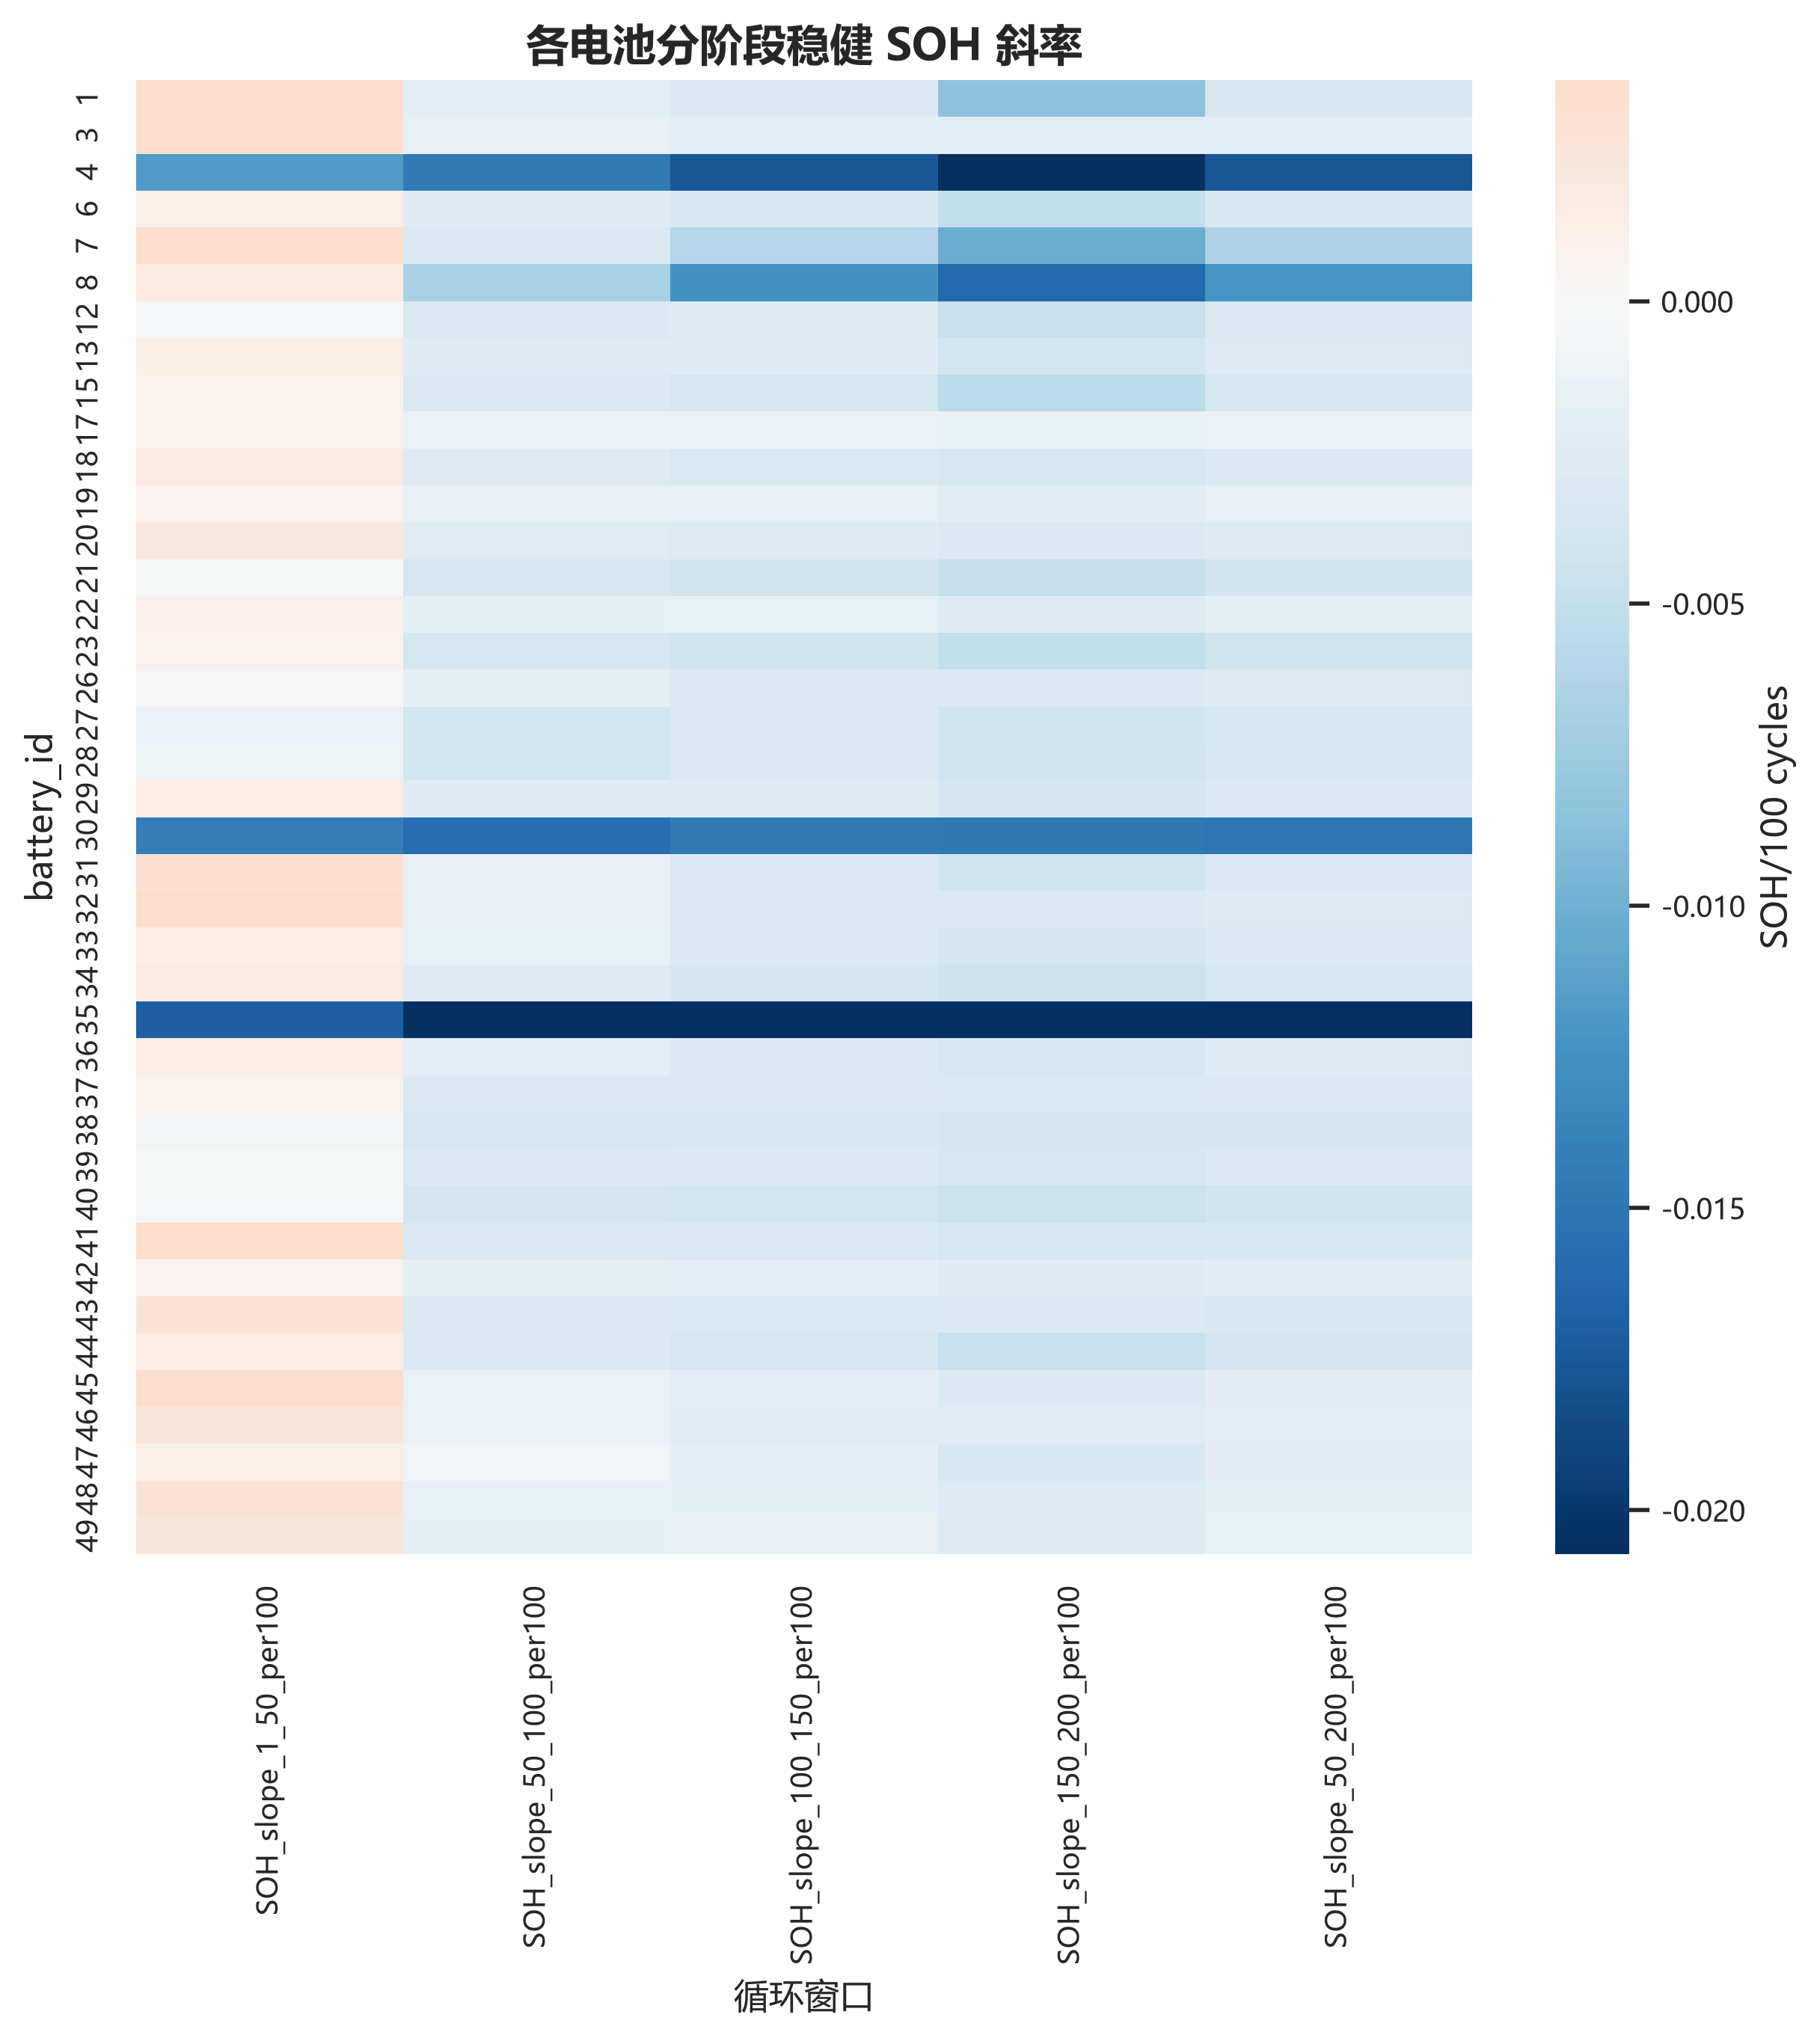
\includegraphics[width=0.62\textwidth]{q1_04_phase_slope_heatmap.png}
\caption{40 块训练电池的分阶段稳健 SOH 斜率}
\label{fig:phase}
\end{figure}

\section{问题一：统一二次退化函数的识别}

\subsection{候选模型与时间截断验证}

保留线性、受约束二次、幂律与指数四类低参数模型。最终模型为
\begin{equation}
  \widehat{\SOH}_i(n)=a_i-d_{1i}x-d_{2i}x^2,
  \qquad x=n/100,\qquad d_{1i},d_{2i}\geq0 .
  \label{eq:quadratic}
\end{equation}
参数通过 soft-$L_1$ 稳健最小二乘得到。模型选择不依赖前 200 次的拟合 $R^2$，而是分别用前 100、150 次拟合并预测已知未来；综合 MAE、RMSE、最大误差、趋势方向、EOL 覆盖和截断寿命稳定性。二次模型兼顾短期外推、单调性与解析寿命，故作为唯一最终函数。其 EOL 为
\begin{equation}
 L=\begin{cases}
 100\dfrac{-d_1+\sqrt{d_1^2+4d_2(a-0.8)}}{2d_2},&d_2>\varepsilon,\\[0.8em]
 100\dfrac{a-0.8}{d_1},&d_2\leq\varepsilon,\ d_1>0.
 \end{cases}
 \label{eq:eol}
\end{equation}
若合理上限内无交点，则标记为无界而不强行给出寿命。

\subsection{参数可辨识性}

对每块电池输出 $a,d_1,d_2$、拟合 RMSE、二次 EOL、边界命中与状态，并进行 300 次移动块残差 bootstrap。跨电池的 $d_1,d_2$ 相关只有 0.025，但单电池 bootstrap 相关系数中位数为 $-0.921$；15/40 电池至少一个参数命中零边界。这说明不同电池的点估计未呈整体负相关，并不能消除同一电池内部的参数补偿。

图\ref{fig:identifiability} 展示了原生参数的零边界聚集。100 次相对 200 次拟合时，$d_1,d_2$ 的中位相对变化分别为 0.143 和 0.430；150 次时降为 0.056 和 0.095。由于约束边界和 bootstrap 补偿明显，后续策略响应改用 $\Rone$ 与 $A$。该变换不改变寿命函数：$d_2=A/2$，$d_1=\Rone-A$，预测后再投影到非负物理域。

\begin{figure}[H]
\centering
\begin{subfigure}{0.48\textwidth}
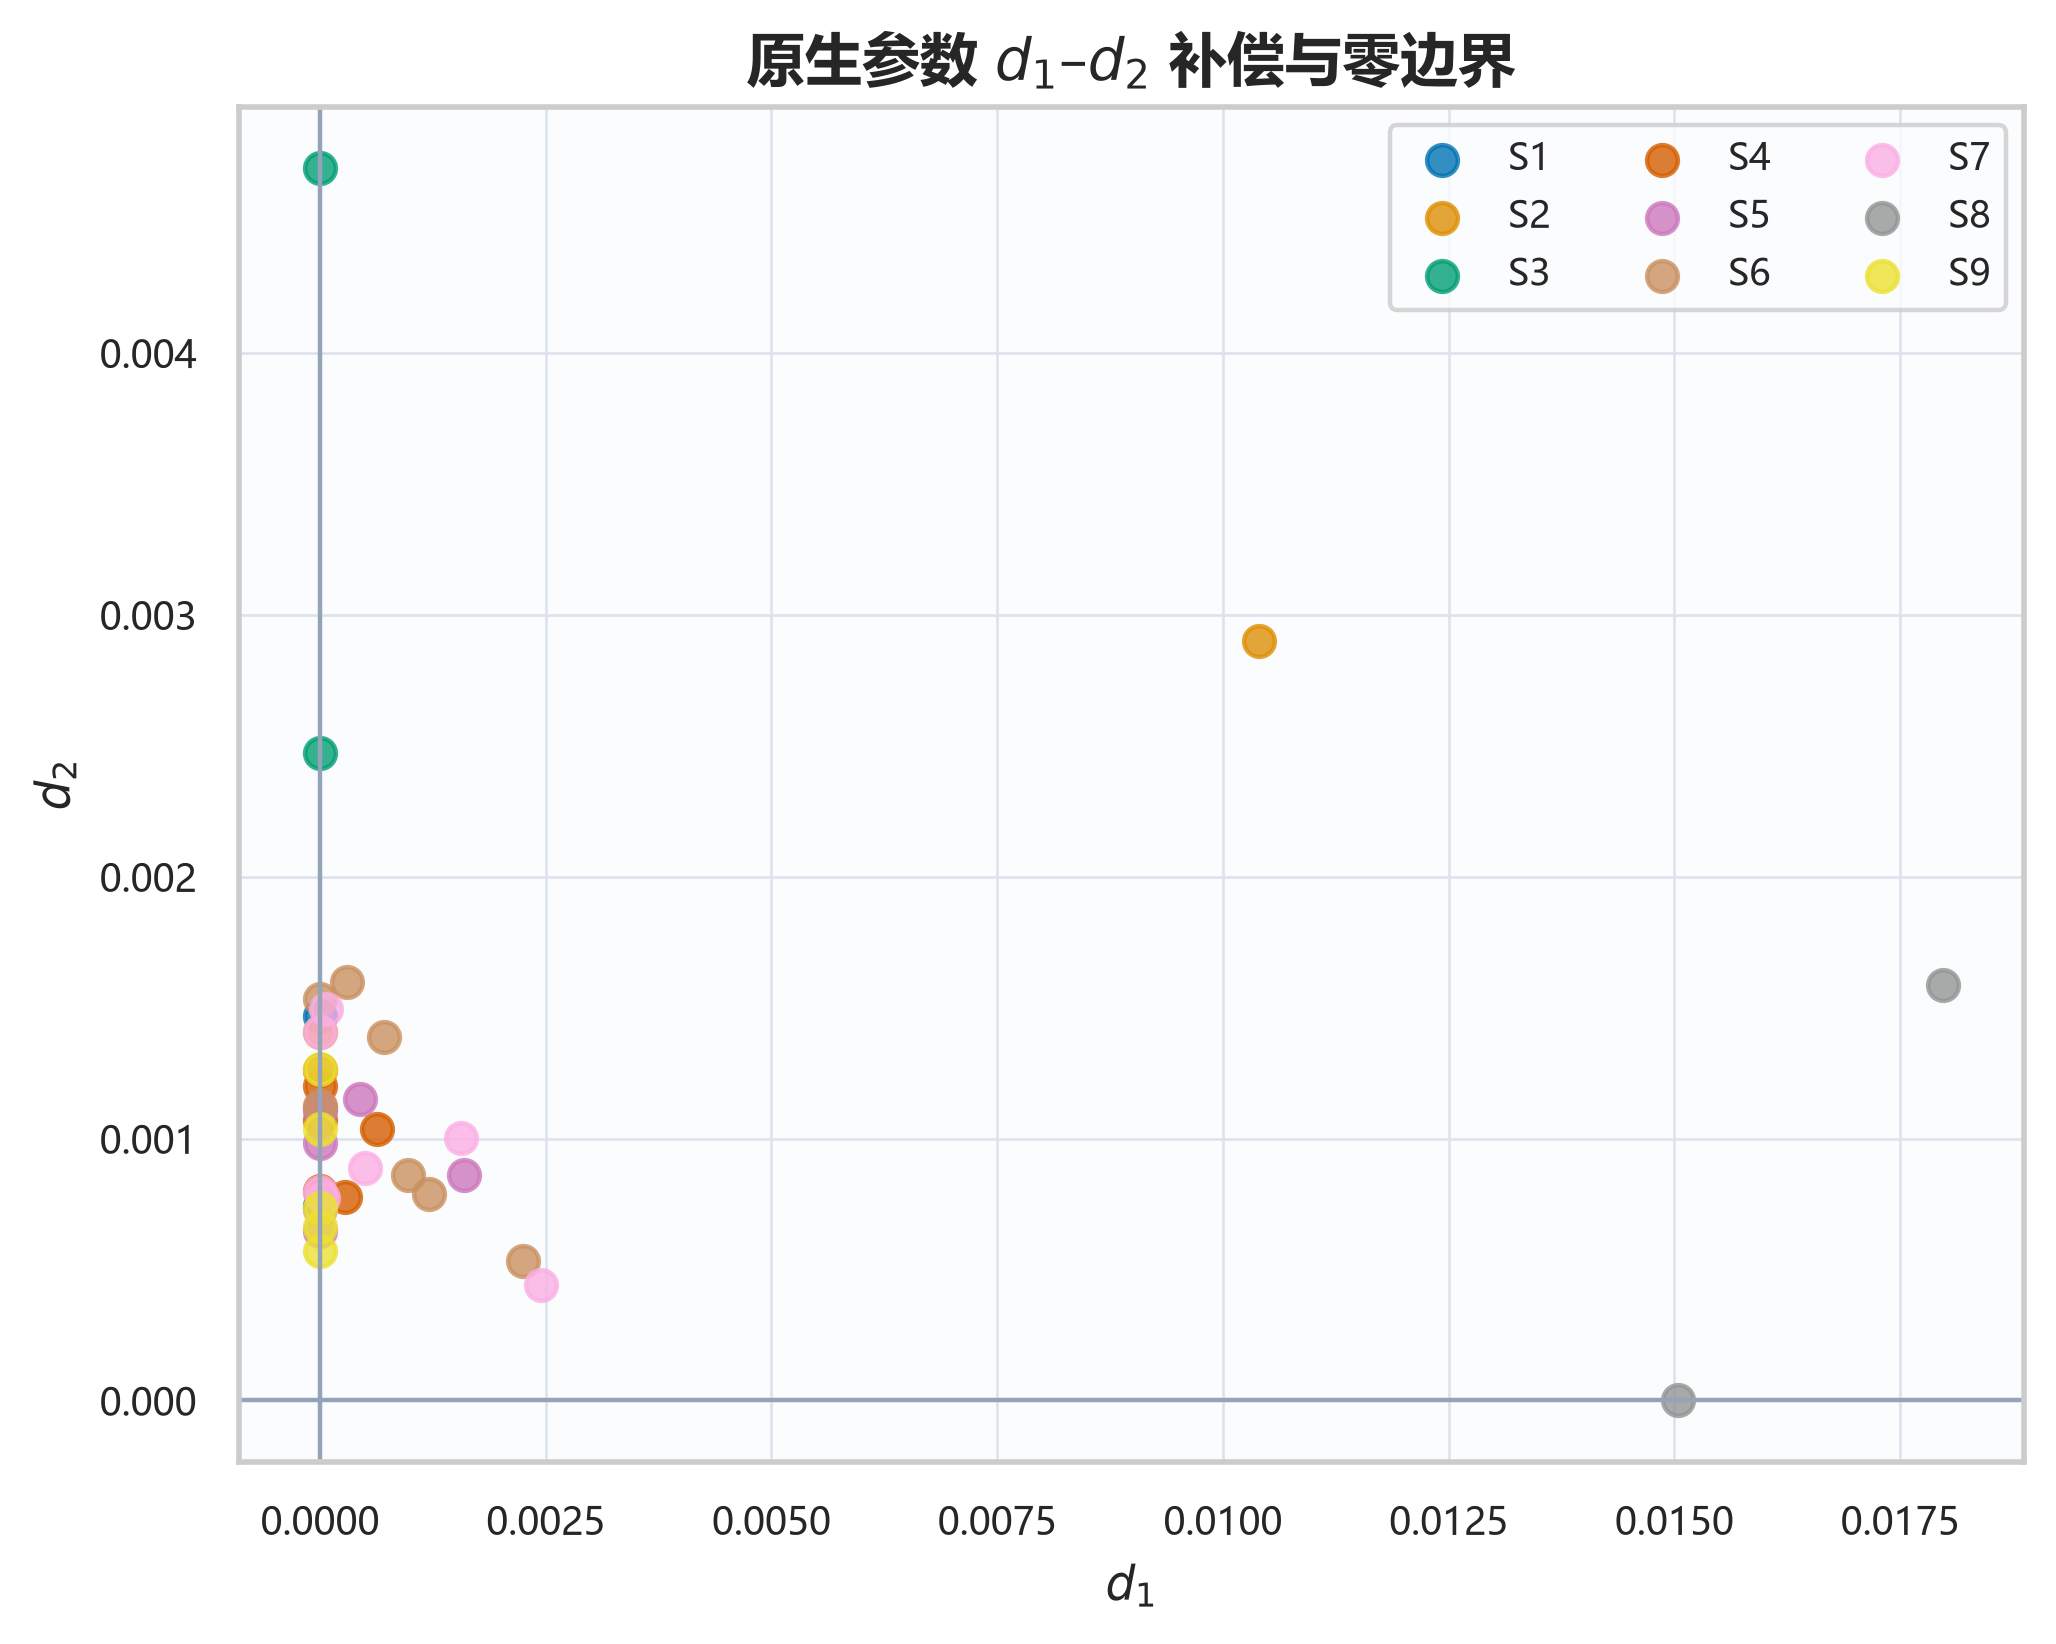
\includegraphics[width=\textwidth]{q1_02_d1_d2_compensation.png}
\caption{原生参数及零边界}
\end{subfigure}\hfill
\begin{subfigure}{0.48\textwidth}
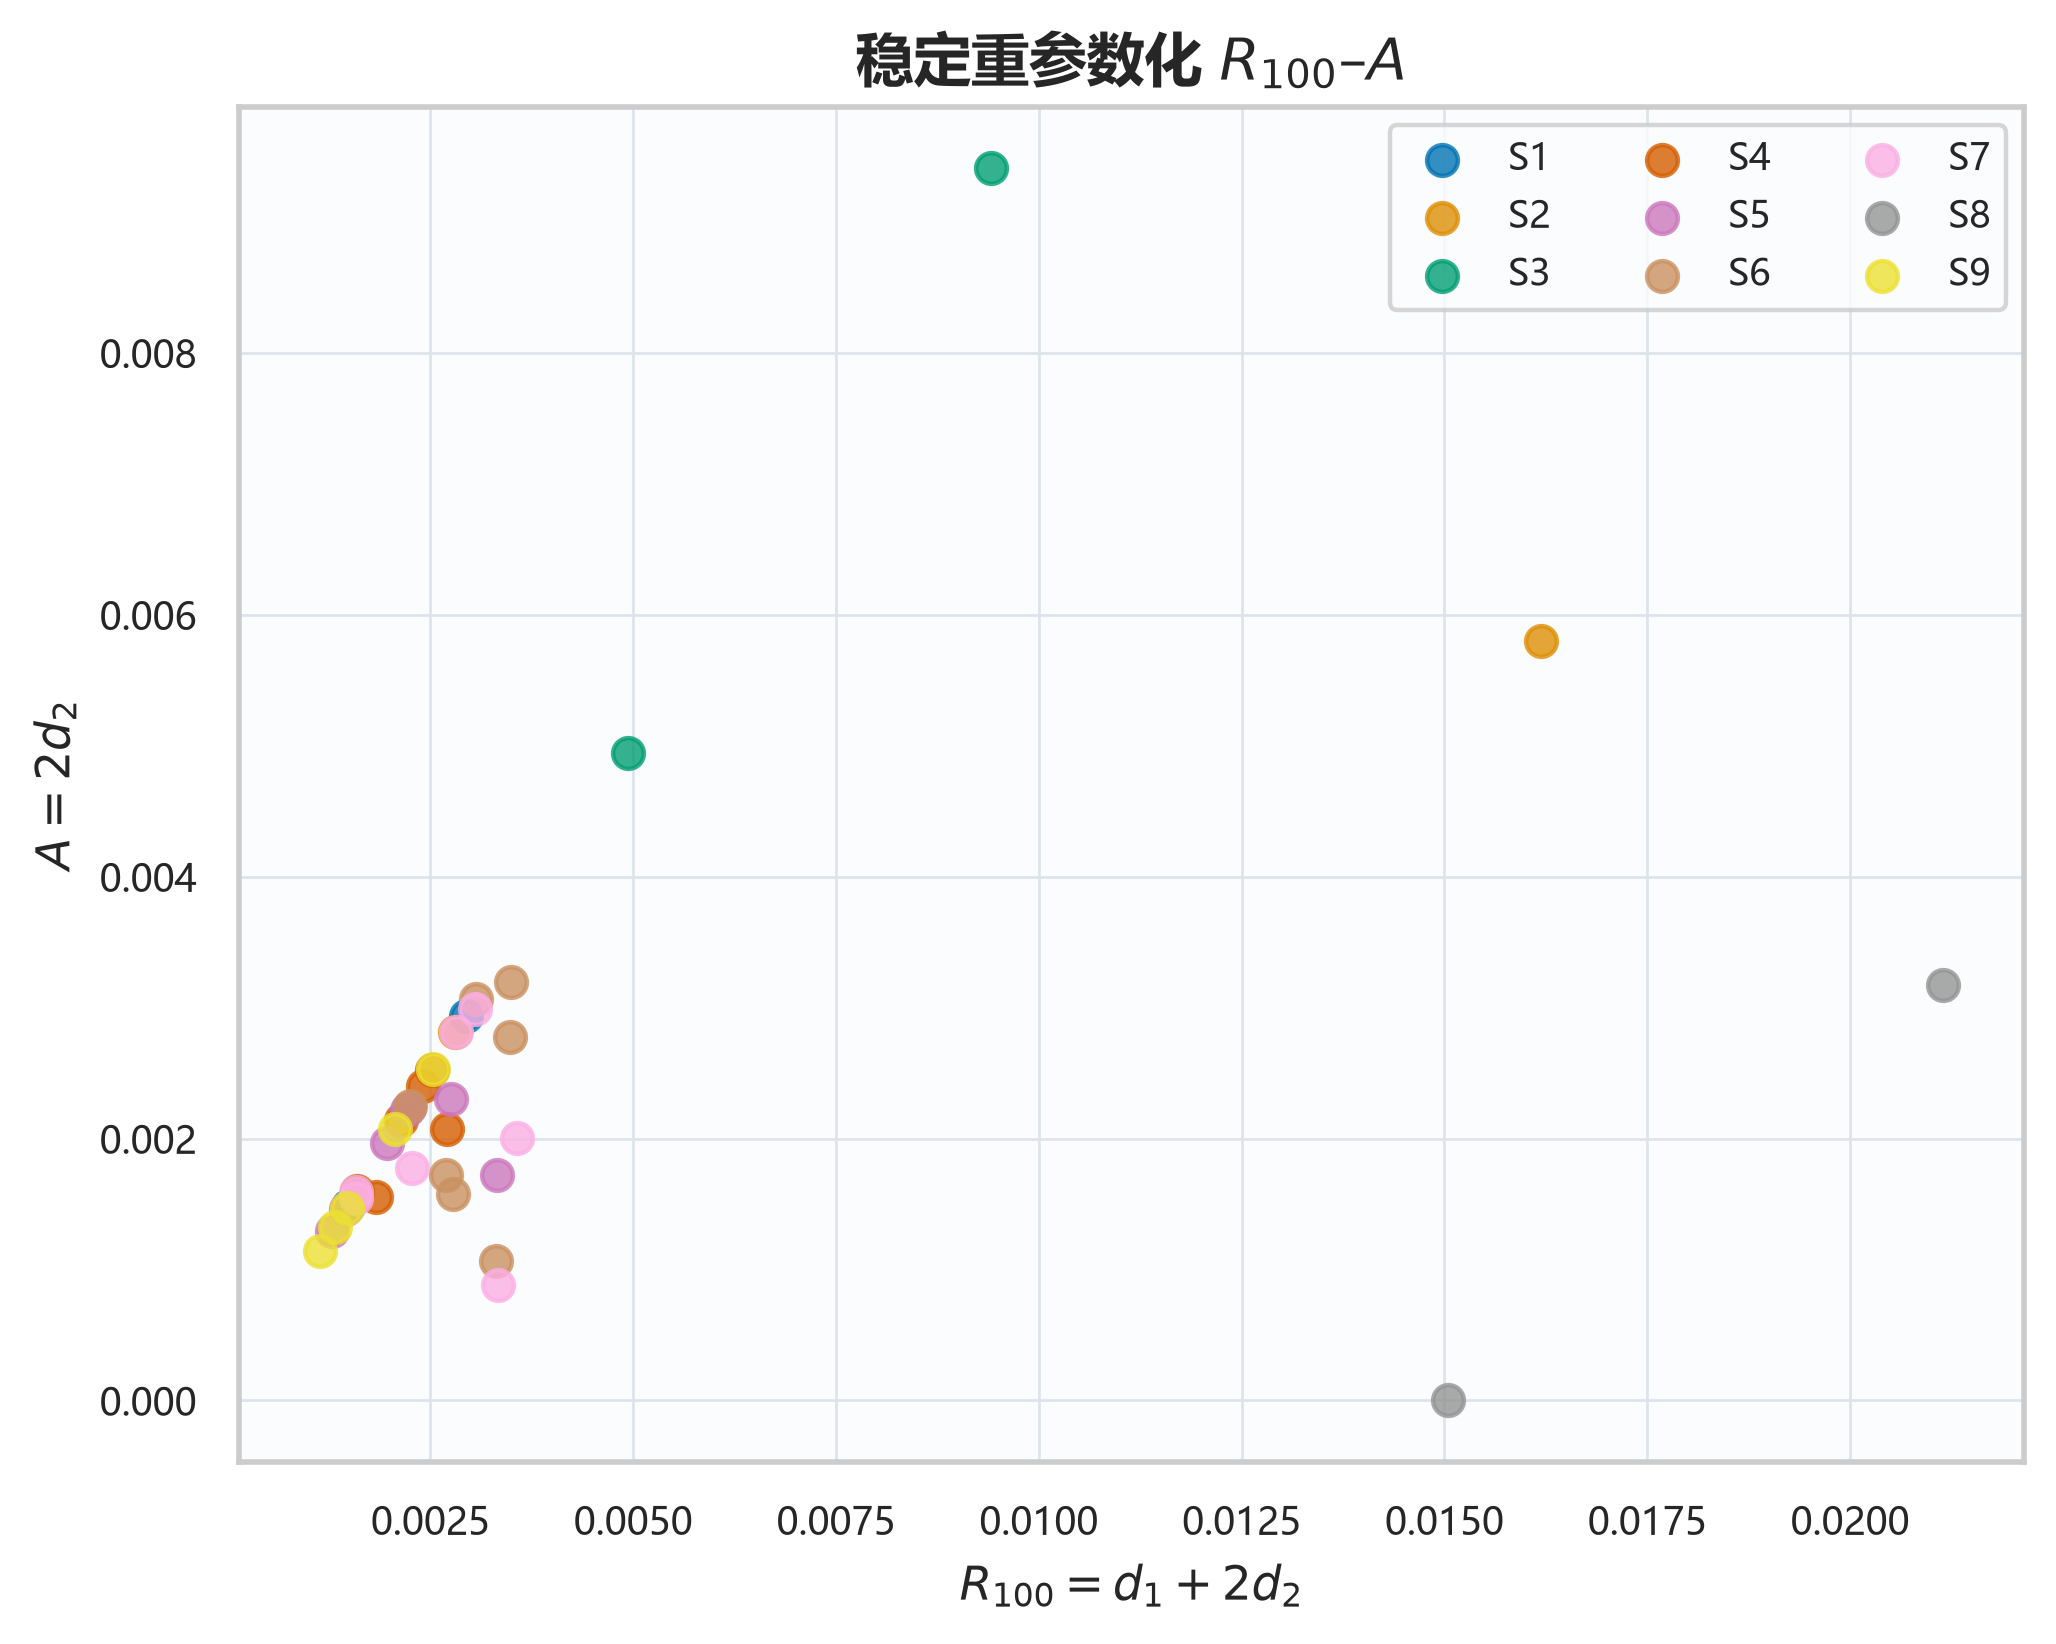
\includegraphics[width=\textwidth]{q1_s01_R100_A_scatter.png}
\caption{稳定重参数化}
\end{subfigure}
\caption{二次参数的可辨识性诊断}
\label{fig:identifiability}
\end{figure}

需要强调：$A=2d_2$ 仍与 $d_2$ 等价，并不会凭变换凭空增加信息；选择 $\Rone,A$ 的主要理由是 $\Rone$ 对 100 次附近的观测局部速率更直接，且能降低对“截距斜率如何分摊”的解释风险。EOL 仍保留明显的长期结构不确定性。

\section{问题二：策略到二次退化参数的桥接}

\subsection{策略级设计与批次控制}

主连续模型限于 dataset 3 的 S4--S9，共 6 个独立 NEWSTRUCTURE 策略点；电池级数据仅用于同策略方差和分组 bootstrap。S2 的 $C_1$ 缺失，完整三参数模型中剔除而不填补。S3 与 S9 具有相同 $(4.8,80,4.8)$，但分属不同结构和批次，其 $A$、SOH$_{200}$ 和 EOL 明显不同，因此单独作为结构--批次对照，而不并入主响应面。

\subsection{原始三参数与两阶段暴露模型}

先比较标准化描述模型
\[
  Y=\beta_0+\beta_1C_1+\beta_2Q_1+\beta_3C_2+\epsilon,
  \qquad Y\in\{\Rone,A\}.
\]
OLS 只报告方向，Ridge 在 LOSO 中选择正则强度。再定义
\[
 q=Q_1/80,\qquad E_1(p)=qC_1^p,\qquad E_2(p)=(1-q)C_2^p,
\]
对 $p\in\{1,1.5,2,2.5,3\}$ 分别拟合 $(E_1,E_2)\to(\Rone,A)$。$E_1+E_2$ 只作旧 stress benchmark，不作为主阶段解释。

\begin{table}[H]
\centering
\caption{策略参数桥接模型的 LOSO 比较}
\begin{tabular}{lccc}
\toprule
模型 & 最优 $p$ & Ridge $\alpha$ & 两响应平均归一化 RMSE \\
\midrule
原始 $C_1,Q_1,C_2$ & -- & 10 & 1.142 \\
两阶段分离暴露 $E_1,E_2$ & 1 & 10 & 1.302 \\
求和 SOC stress benchmark & 3 & 10 & 1.229 \\
\bottomrule
\end{tabular}
\label{tab:q2cv}
\end{table}

原始三参数模型虽在三者中最好，但归一化 RMSE 仍大于 1，意味着它没有稳定优于折内均值。故选择它只是“当前候选中相对较少损失且能直接输出参数”，不是强泛化证据。图\ref{fig:q2models} 也显示留一预测对 S8、S9 等点较敏感。

\begin{figure}[H]
\centering
\begin{subfigure}{0.48\textwidth}
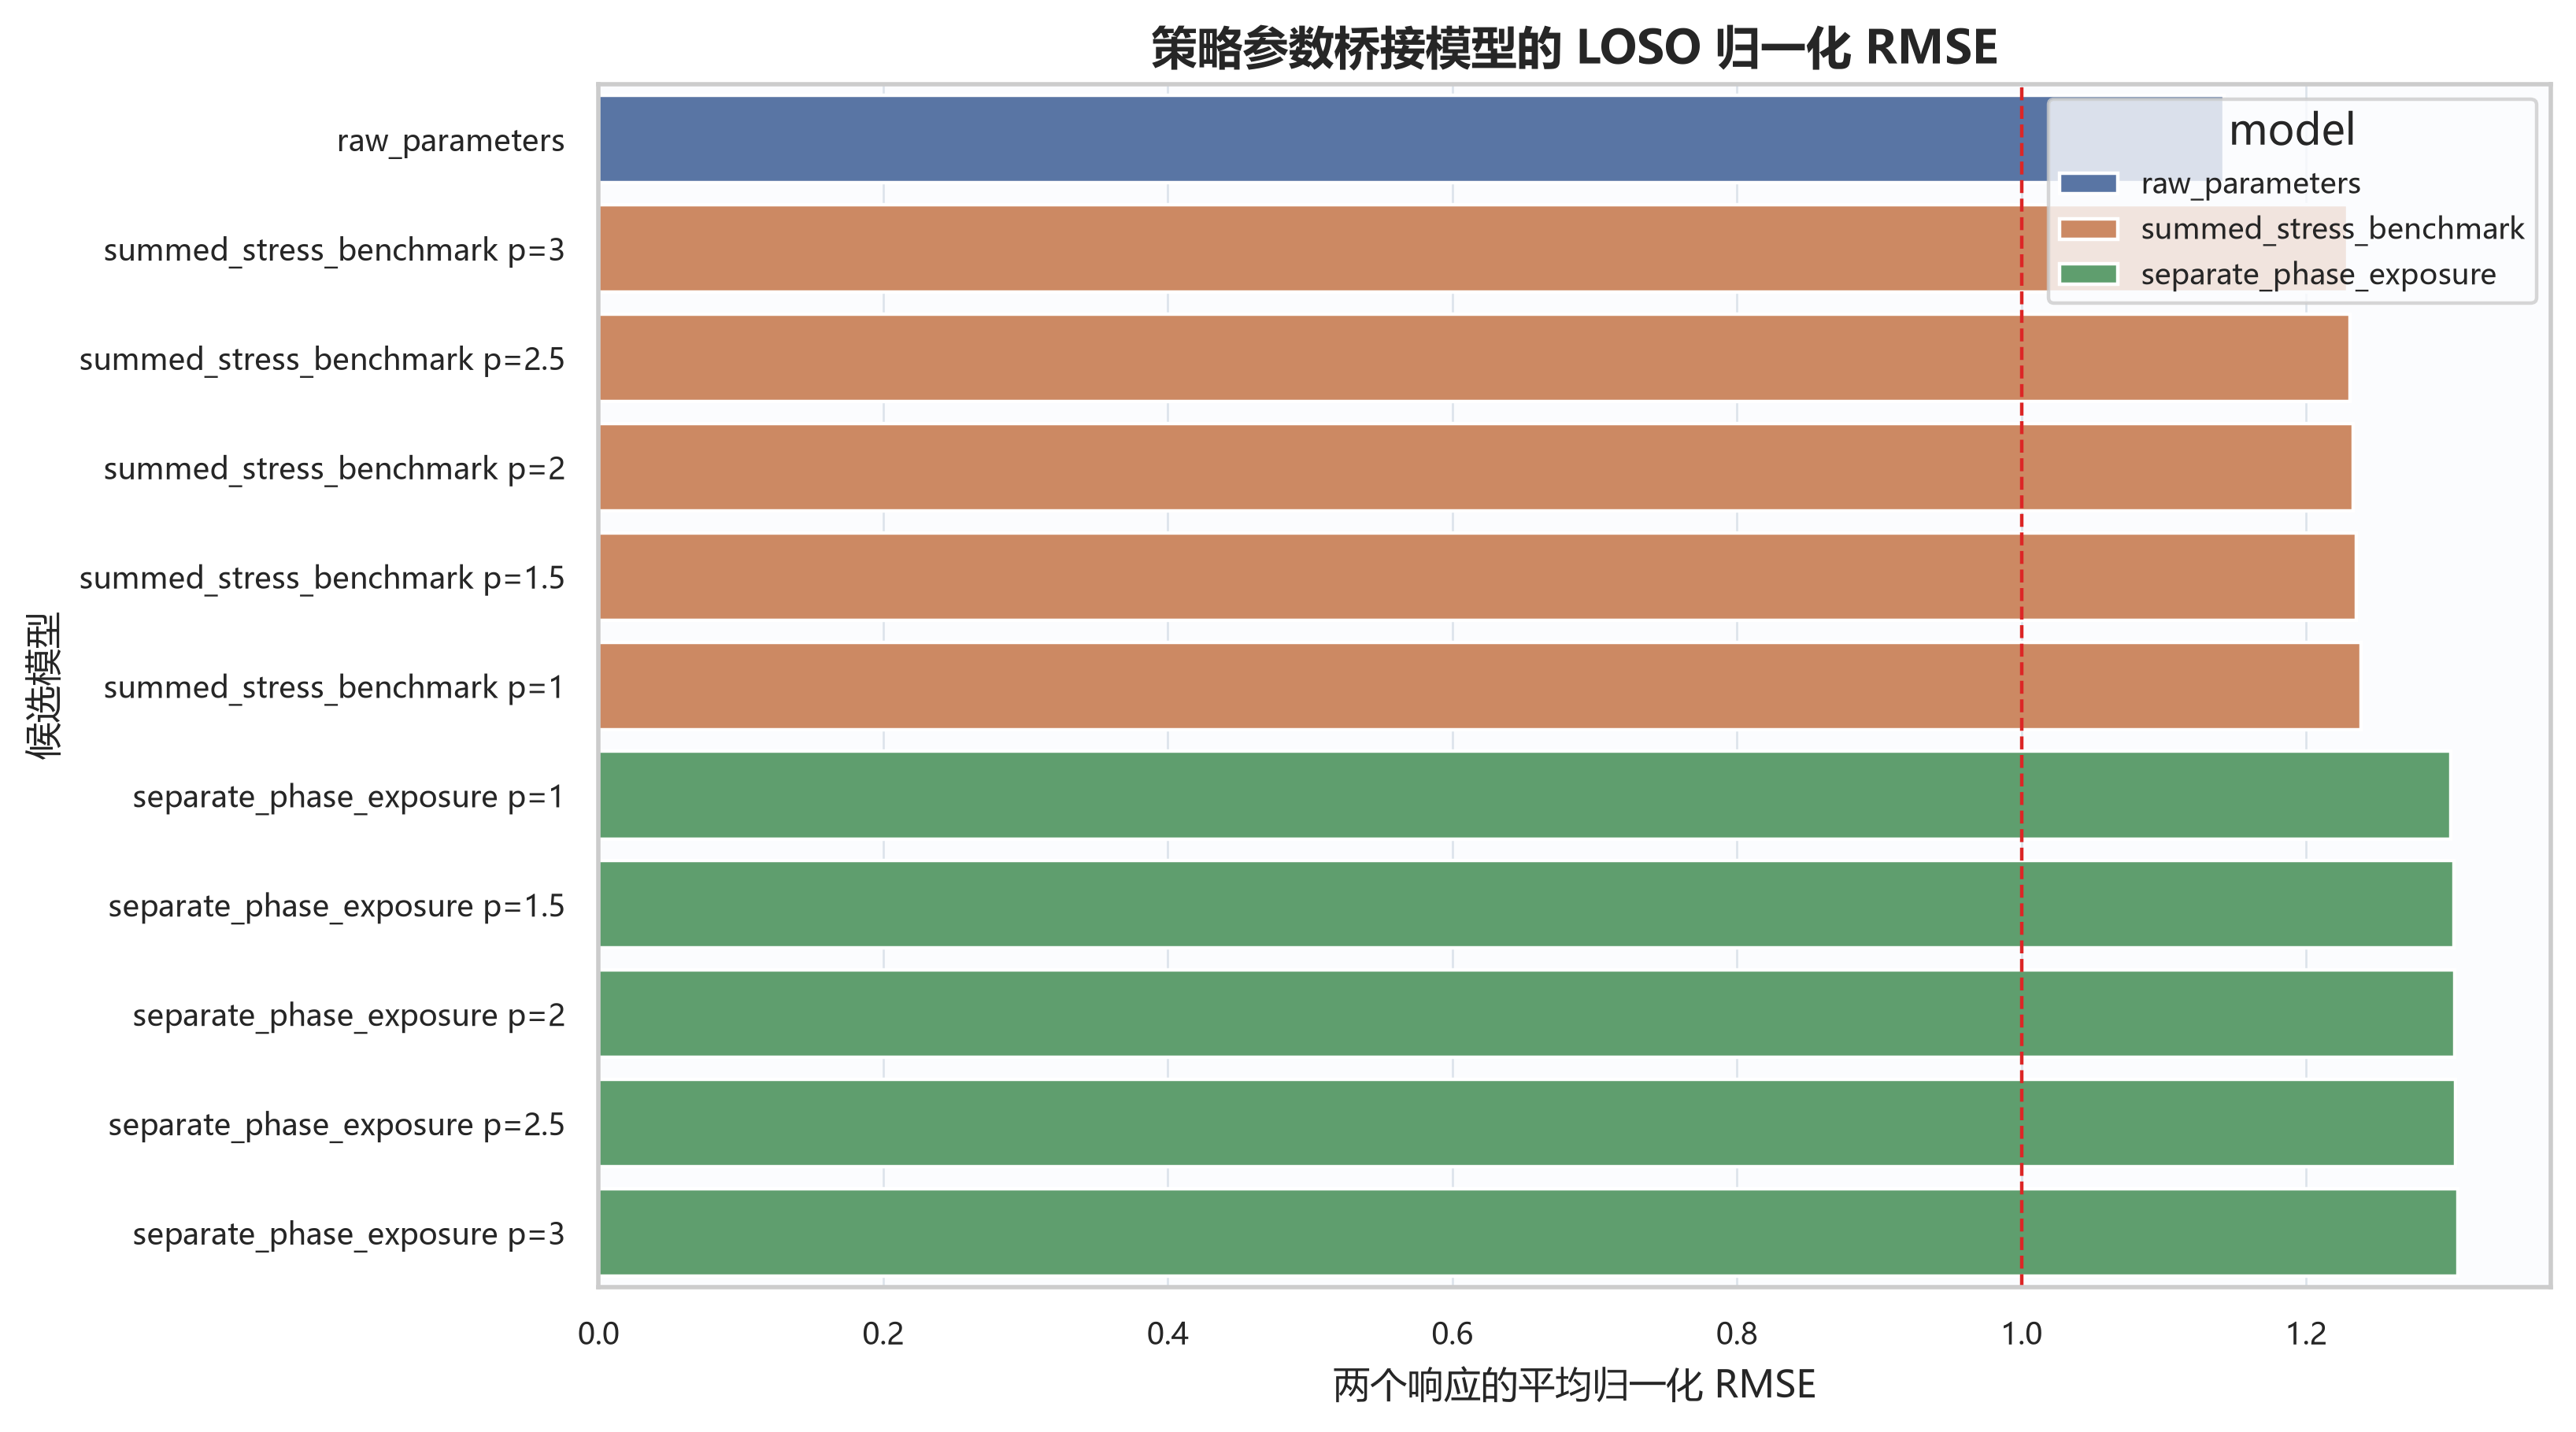
\includegraphics[width=\textwidth]{q2_06_strategy_model_loso.png}
\caption{候选模型 LOSO}
\end{subfigure}\hfill
\begin{subfigure}{0.48\textwidth}
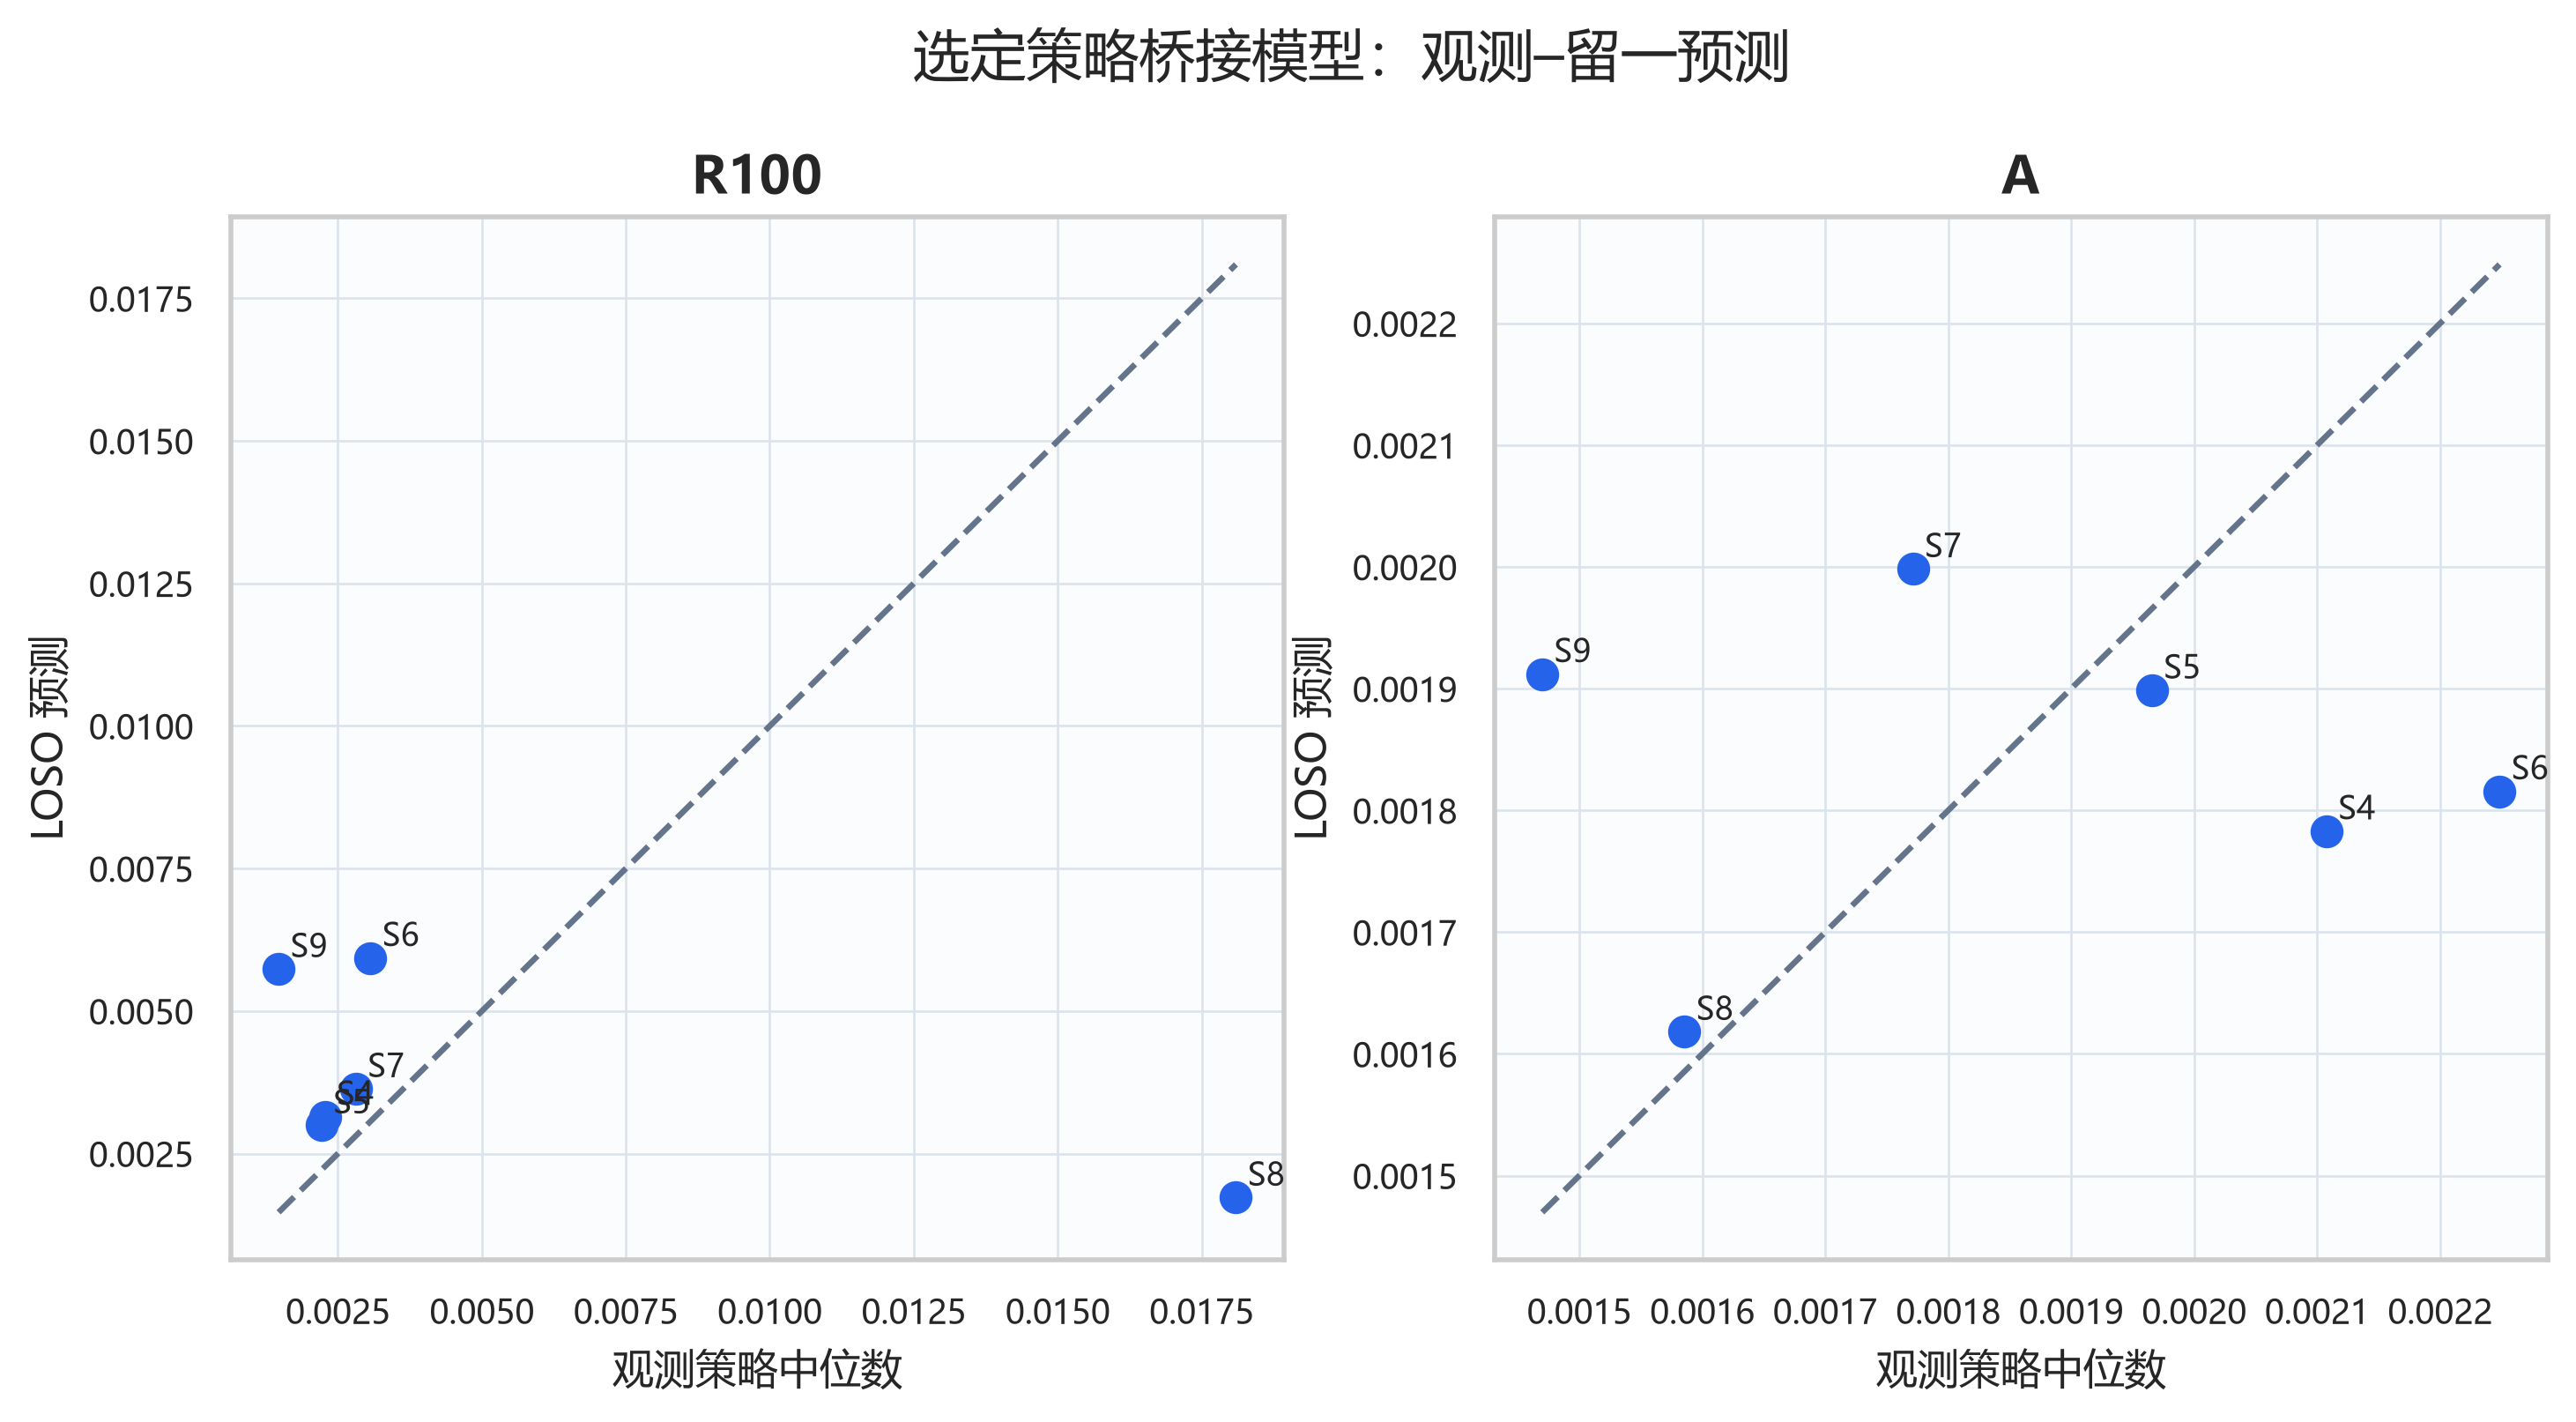
\includegraphics[width=\textwidth]{q2_07_selected_model_observed_predicted.png}
\caption{观测与留一预测}
\end{subfigure}
\caption{策略到退化参数桥接的泛化检验}
\label{fig:q2models}
\end{figure}

1000 次“先抽策略、再抽策略内电池”的 bootstrap 中，原始模型只有 $Q_1\to\Rone$ 的区间不跨 0，方向稳定率为 0.992。两阶段暴露模型中 $E_1\to\Rone$ 为负、$E_2\to\Rone$ 为正，方向稳定率分别为 0.995 与 0.994；但 $E_1,E_2\to A$ 的稳定率只有 0.559 与 0.541，且模型 LOSO 更差。数据因而提示：在本设计邻域内，第二阶段暴露更可能改变 100 次附近的基础速率，而没有证据表明其稳定改变加速度；该判断仍受 6 个策略点和共线性限制，不能推广成物理定律。

\begin{figure}[H]
\centering
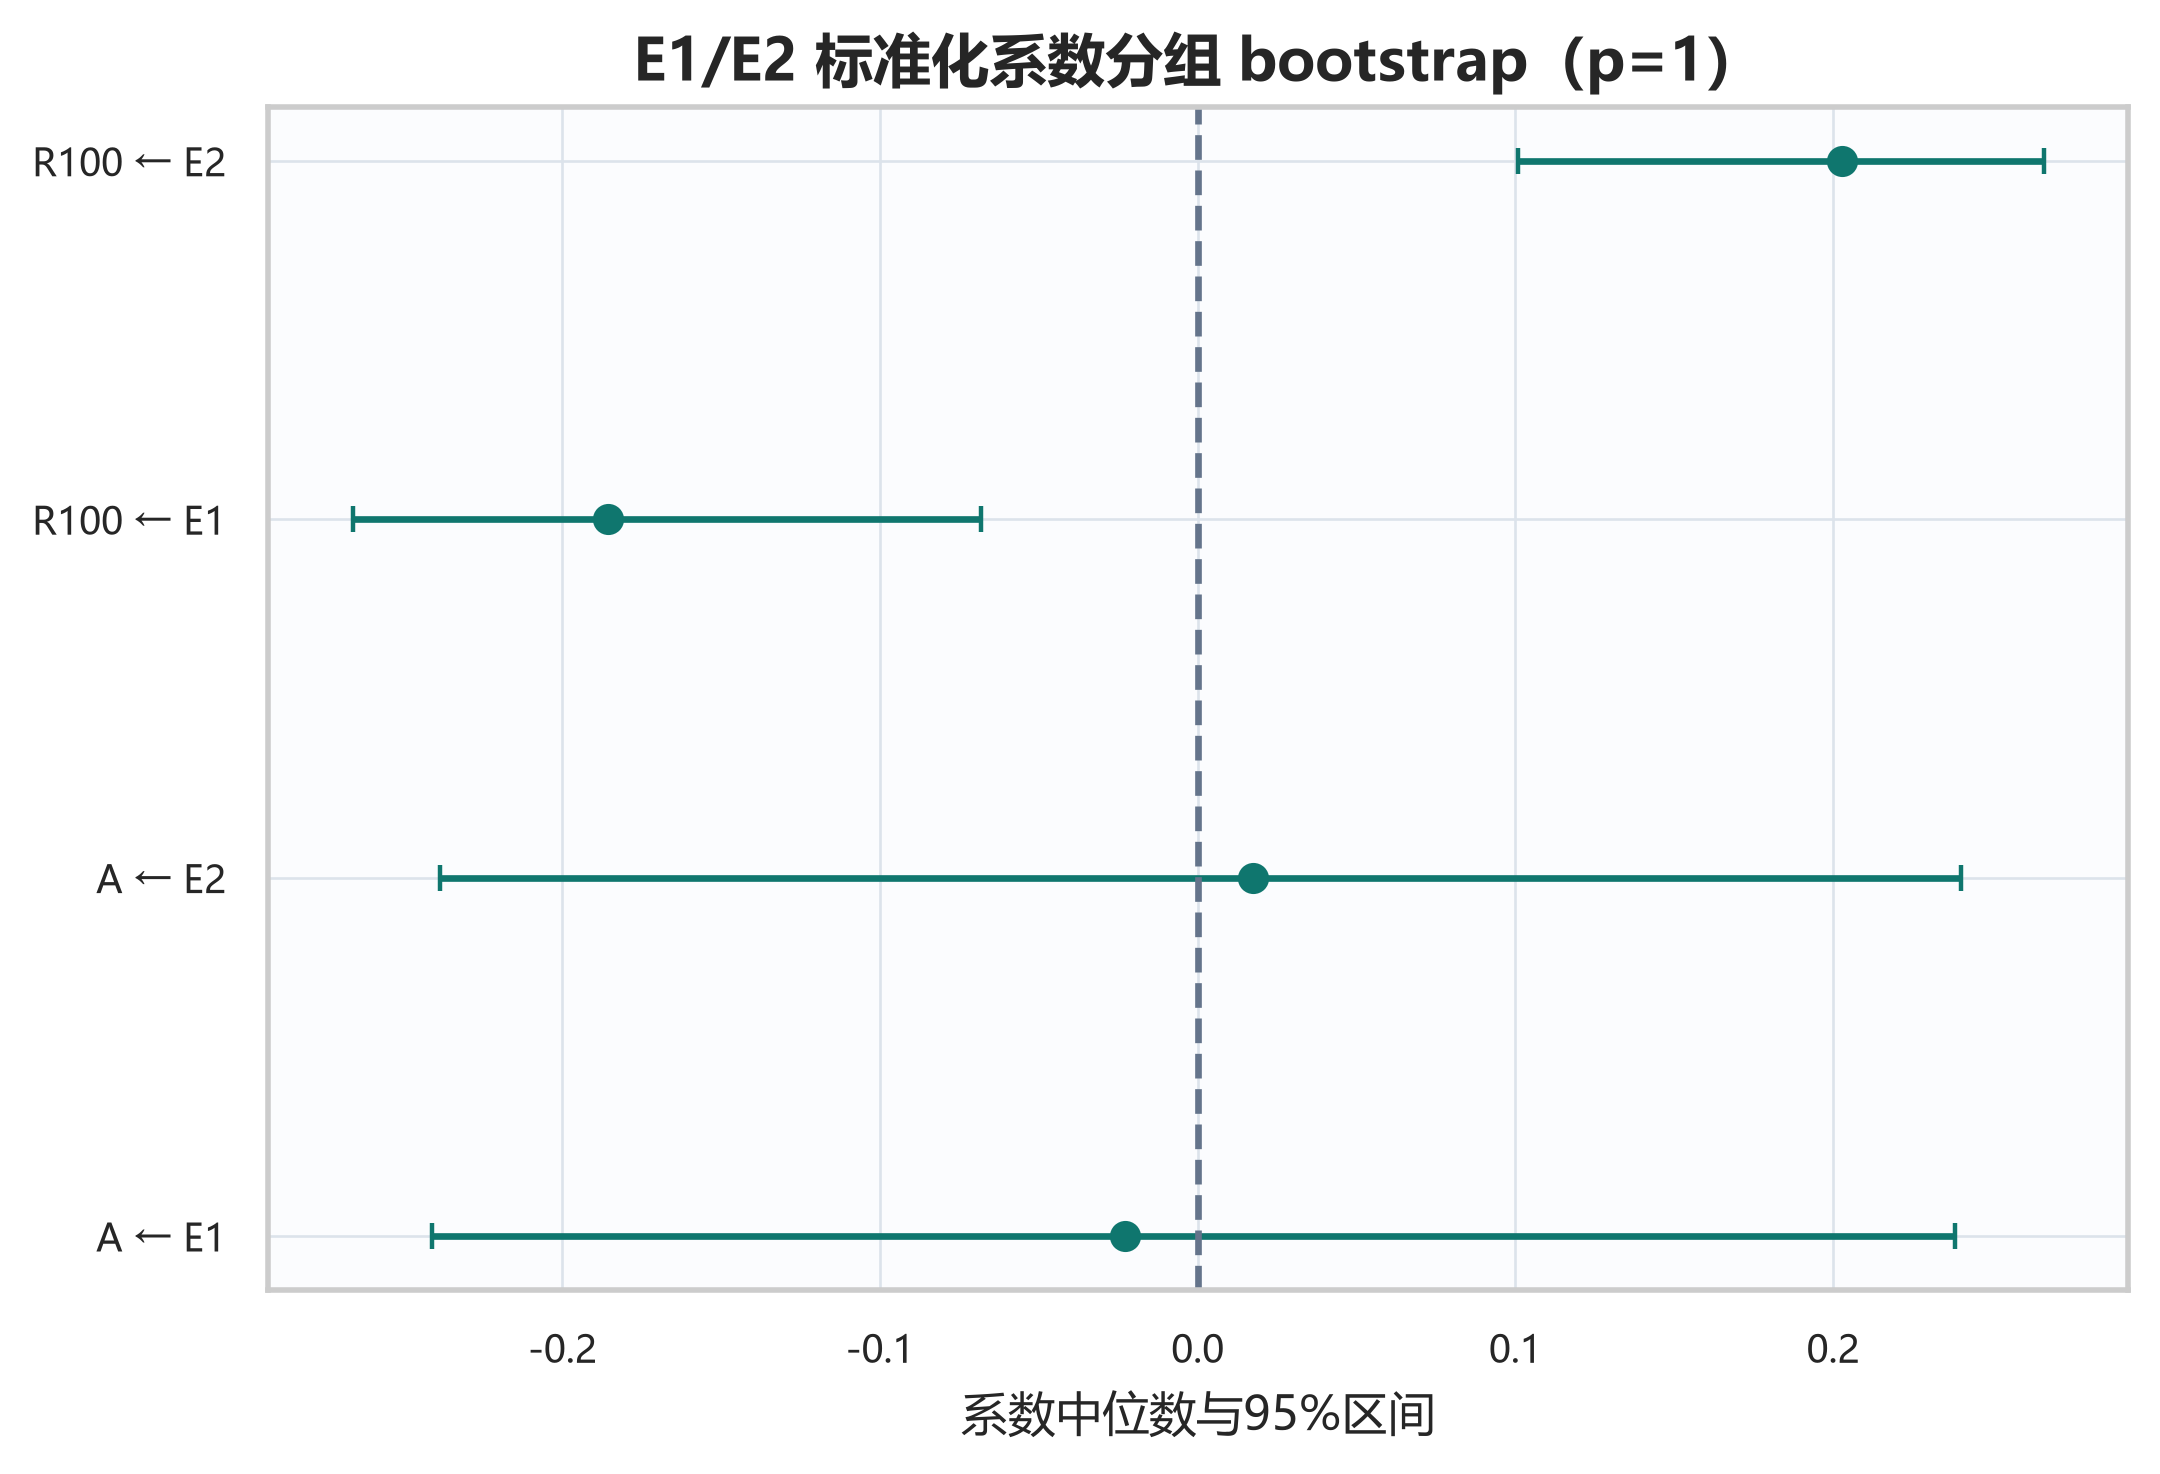
\includegraphics[width=0.72\textwidth]{q2_s03_exposure_coefficient_forest.png}
\caption{两阶段暴露模型的标准化系数与策略优先 bootstrap 区间}
\end{figure}

\subsection{回映寿命、机制关联与证据分级}

对每个策略的预测 $\widehat\Rone,\widehat A$ 先转回非负 $\widehat d_1,\widehat d_2$，令 $a_{\rm ref}=1$，再由式\eqref{eq:eol} 求 EOL。dataset 3 已观测策略的 $a=1$ EOL 重现 MAE 为 118 次，说明桥接误差不能忽略。S3--S9 对照进一步证明结构或批次变量未被三个充电参数完全解释。

机制关联只使用第 1--50 次的 IR、温度和充电时间特征。M0 为策略参数，M1 加初始容量，M2 再加早期健康特征；验证时整种策略留出。对 50--200、100--150、150--200 斜率和 SOH$_{200}$，M2 相对 M1 的中位归一化 RMSE 没有改善，SOH$_{200}$ 甚至从 1.183 增至 1.633。因此没有足够证据称策略效应通过早期阻抗或热状态稳定体现，更不能称为因果中介。

综合直接 SOH/斜率、二次参数桥接、LOSO、bootstrap、局部匹配、早期健康关联和批次敏感性七个通道，$C_1,E_1,E_2$ 总体列为 unsupported；$Q_1,C_2$ 只有 directional but limited。这里的“方向性”主要来自局部趋势或某一响应，并不等于独立显著效应。

\section{问题三：前 150 次预测与个体二次曲线修正}

\subsection{策略先验二次模型}

对目标电池 $i$，策略模型给出 $\mu_{d_1},\mu_{d_2}$ 及策略内尺度 $\sigma_{d_1},\sigma_{d_2}$，用前 150 次稳健 SOH 最小化
\begin{equation}
 \mathcal L_i=\mathcal L_{\rm robust}(y_{i,1:150},\widehat y_i)
 +\lambda\left[\left(\frac{d_{1i}-\mu_{d_1}}{\sigma_{d_1}}\right)^2
 +\left(\frac{d_{2i}-\mu_{d_2}}{\sigma_{d_2}}\right)^2\right].
 \label{eq:prior}
\end{equation}
对训练电池伪测试时，目标电池从策略中位数和策略桥接模型中完整排除。$\lambda$ 在 40 块训练电池的 LOBO 伪测试中选择，而不是手工指定。最终选择为 $\lambda=0$，这等价于拒绝当前稀疏策略先验的收缩收益。保留该结果比强制使用先验更符合无泄漏交叉验证原则。

\subsection{与自适应集成的正式比较}

\begin{table}[H]
\centering
\caption{40 块训练电池 151--200 次严格伪测试}
\small
\begin{tabular}{lccccc}
\toprule
模型 & MAE & RMSE & P90 & 最坏值 & 第 200 次 MAE \\
\midrule
个体 quadratic & 0.000426 & 0.000514 & 0.000869 & 0.003075 & 0.000744 \\
policy quadratic & 0.000505 & 0.000597 & 0.000914 & 0.003452 & 0.000868 \\
adaptive ensemble & \textbf{0.000277} & \textbf{0.000361} & \textbf{0.000901} & \textbf{0.002912} & \textbf{0.000522} \\
\bottomrule
\end{tabular}
\label{tab:q3}
\end{table}

三者趋势方向匹配率均为 1；基于目标电池外残差的点态 95\% 区间覆盖约为 92.8\%。集成模型的平均与最坏误差均占优，故第 151--200 次仍由其负责。早期特征消融中，SOH-only 的点态 RMSE 为 0.000537；加入 IR、温度、充电时间或策略先验后均未稳定下降，因此最终不保留这些高维修正。

\begin{figure}[H]
\centering
\begin{subfigure}{0.48\textwidth}
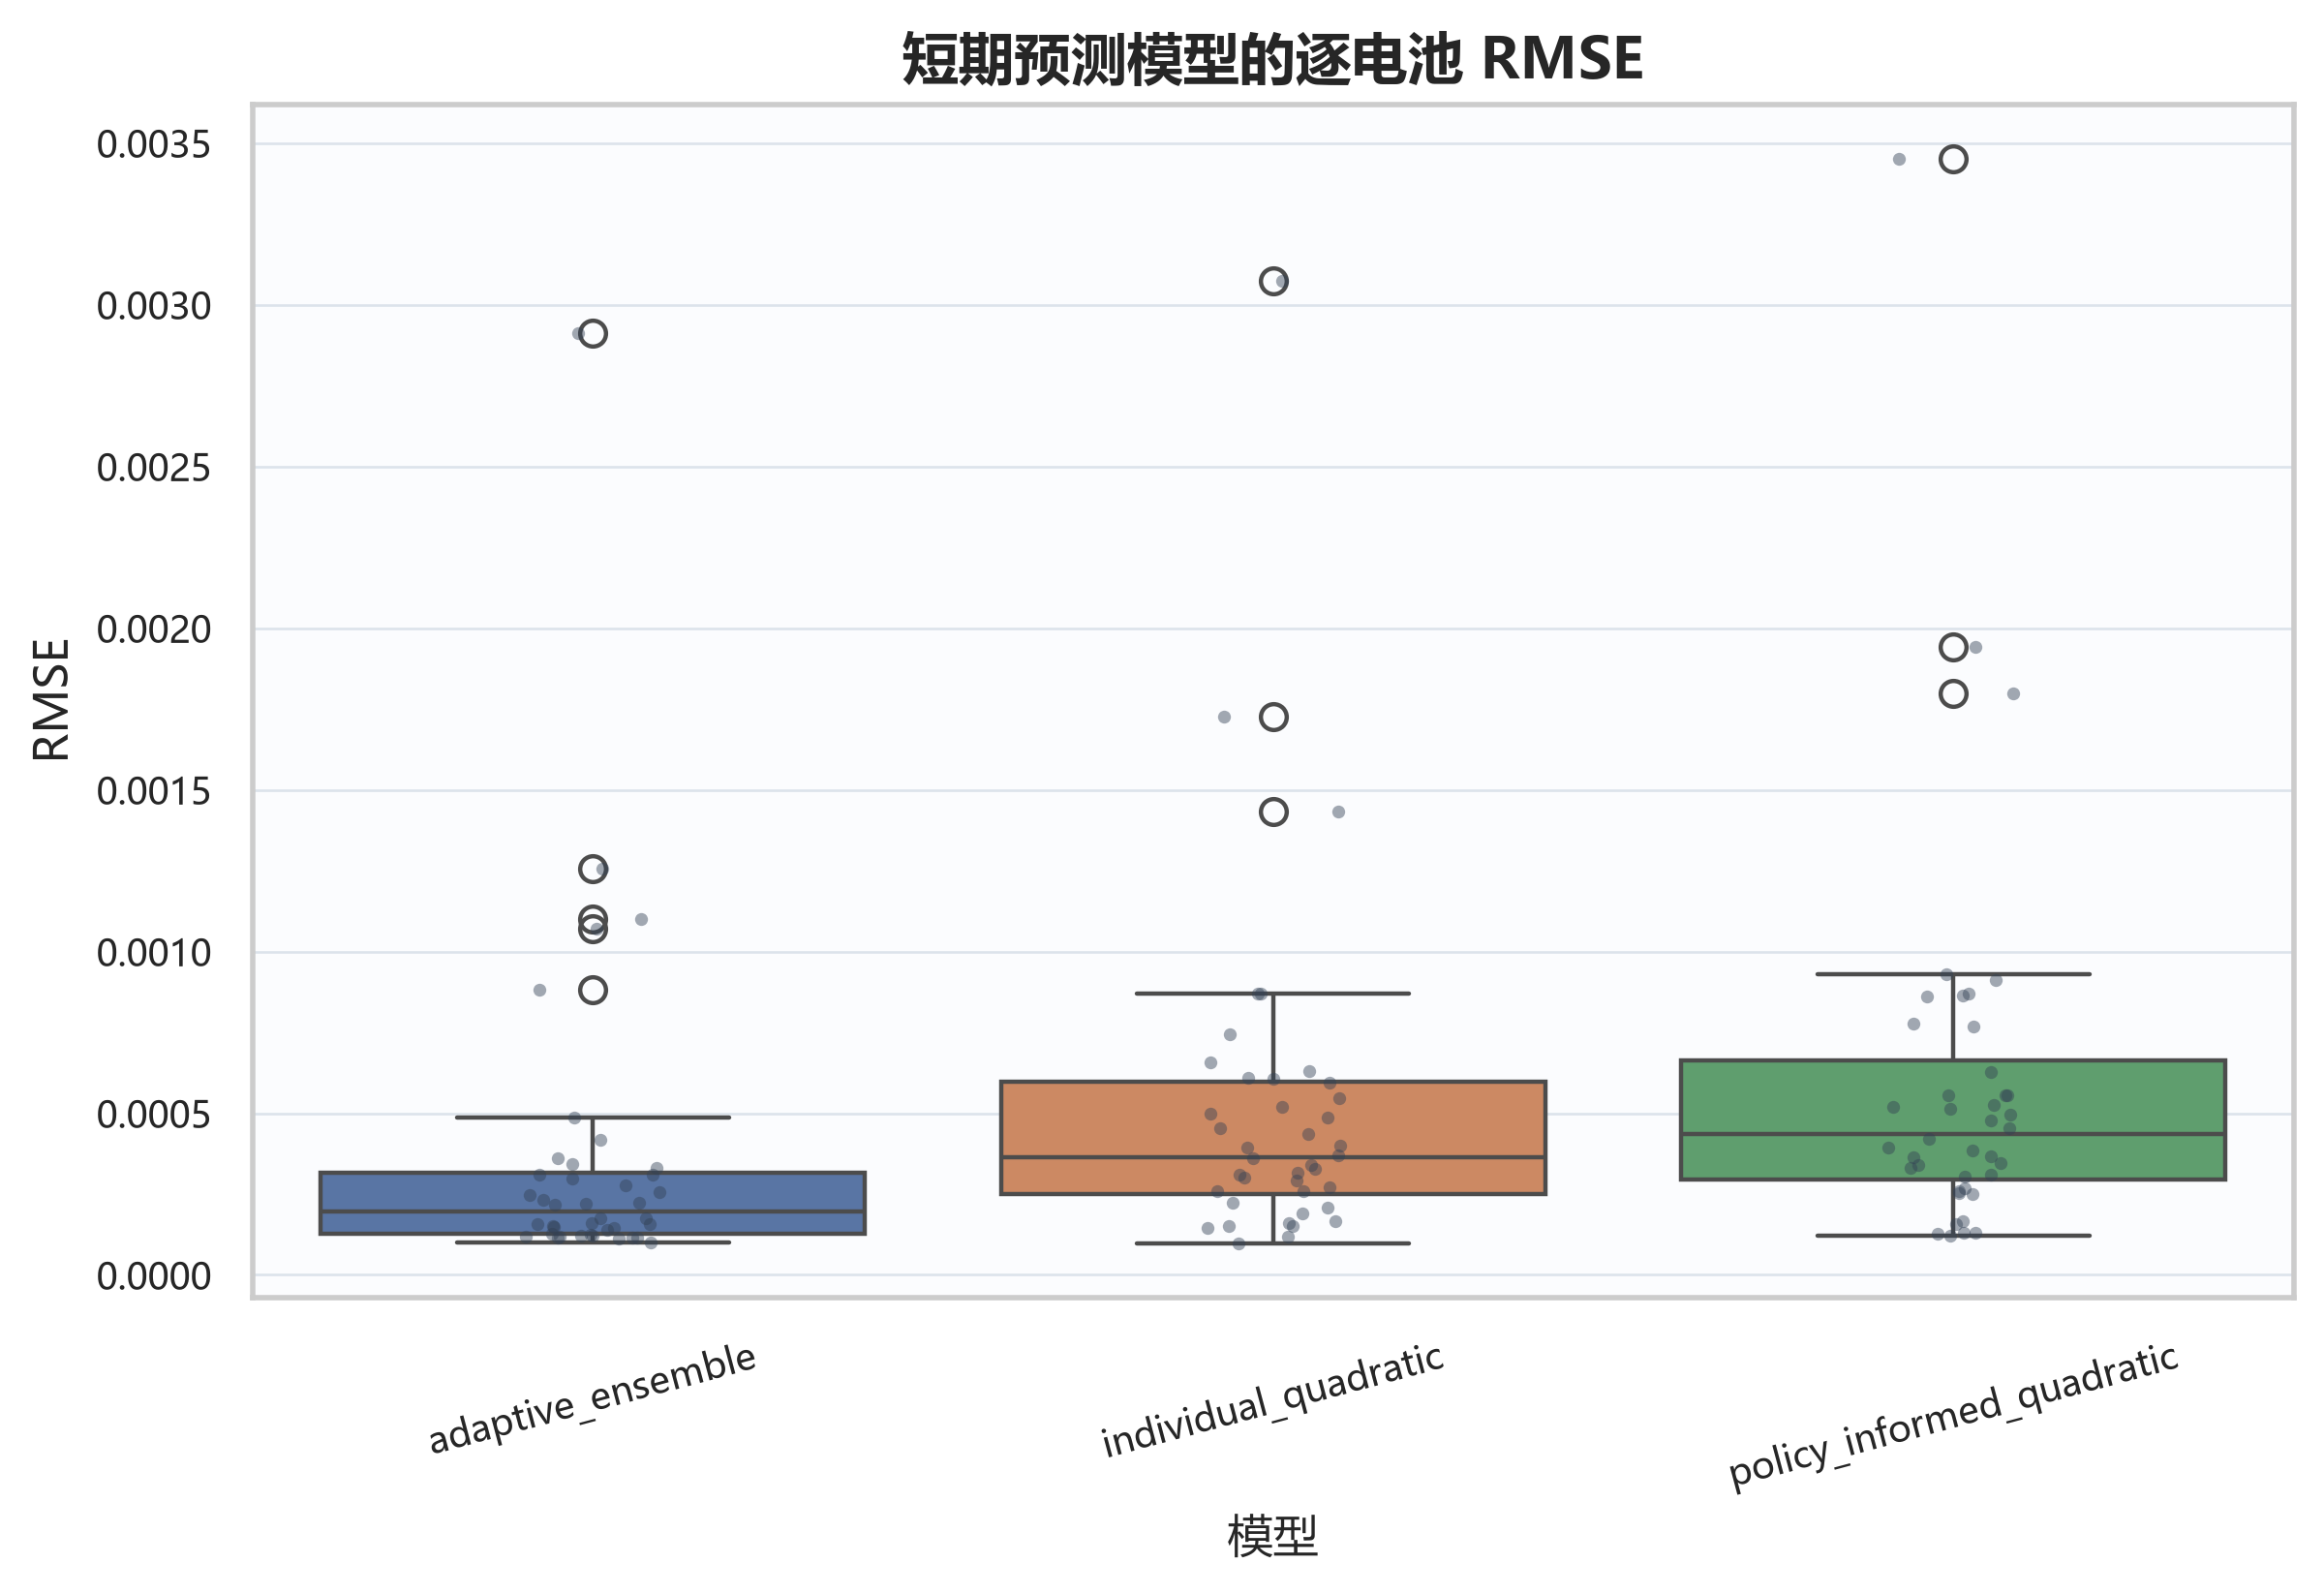
\includegraphics[width=\textwidth]{q3_14_model_rmse_distribution.png}
\caption{逐电池 RMSE}
\end{subfigure}\hfill
\begin{subfigure}{0.48\textwidth}
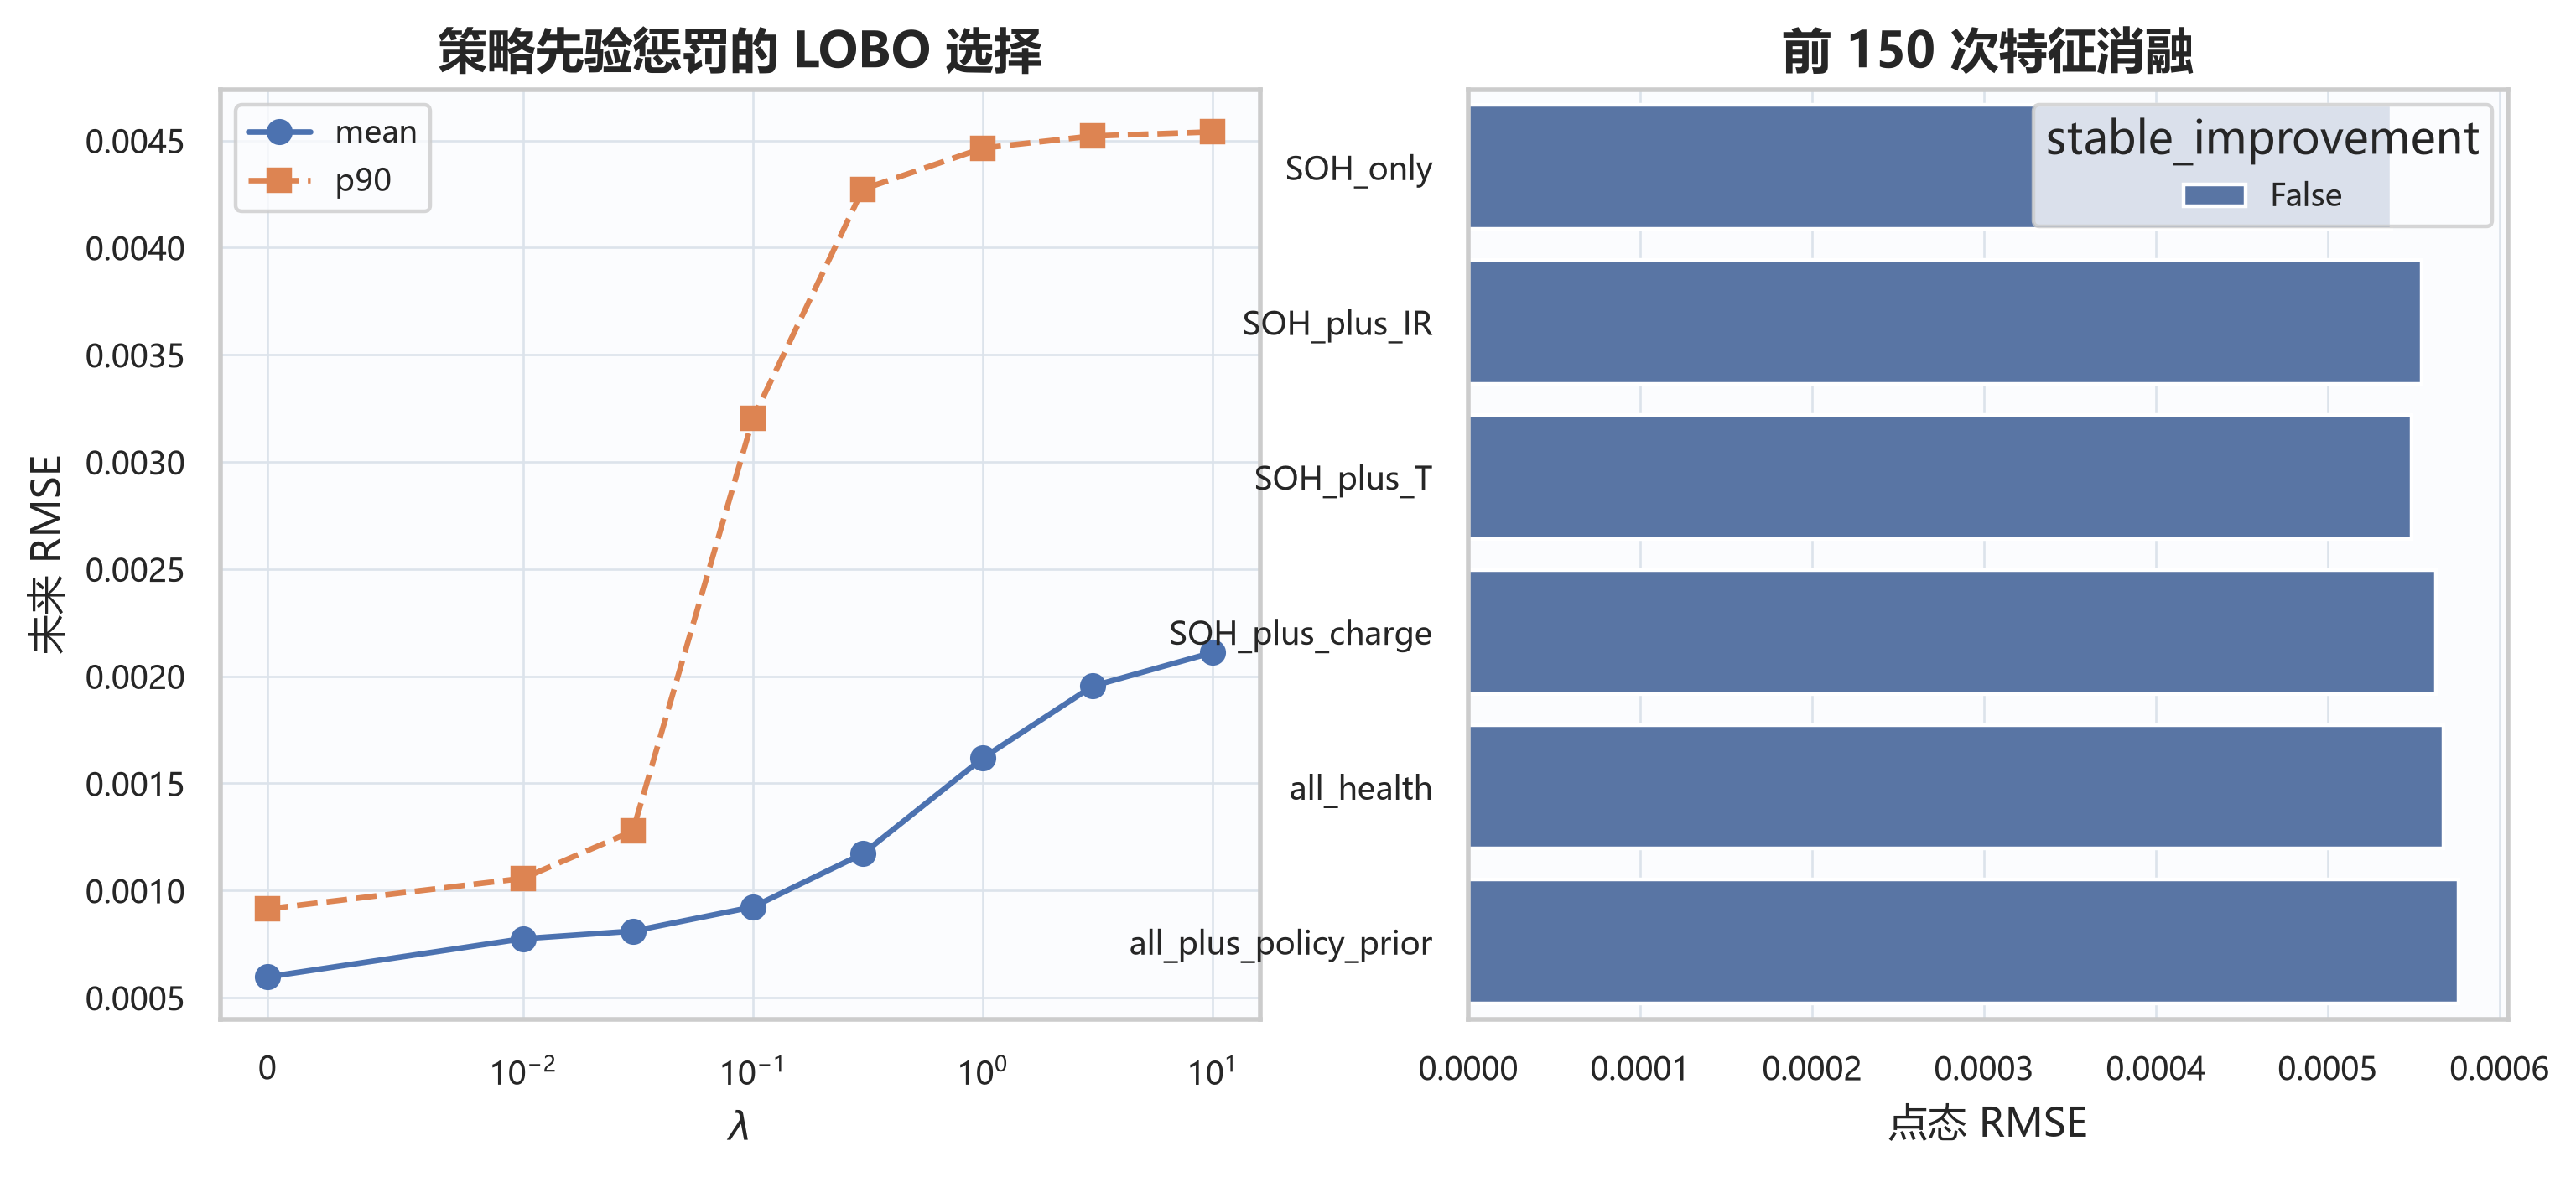
\includegraphics[width=\textwidth]{q3_15_penalty_and_feature_ablation.png}
\caption{先验与特征消融}
\end{subfigure}
\caption{问题三模型选择证据}
\end{figure}

\subsection{测试电池短期预测与统一 EOL}

对 9 块测试电池输出第 151--200 次逐循环预测及区间。然后把第 1--150 次真实轨迹与第 151--200 次选定预测拼接，重新拟合式\eqref{eq:quadratic}，再由式\eqref{eq:eol} 求寿命。该步骤保证短期预测器即使是 ensemble，最终寿命曲线仍只有一个函数。

测试 EOL 点估计约为 661--1547 次。Battery 2 的 95\% bootstrap 区间约为 1373--2776 次，宽度比 0.862，列为 lower；Battery 9、16 的区间较窄，条件可靠性相对更高。9 块电池的寿命都只是模型条件下的外推，不是真实失效标签。

\begin{figure}[H]
\centering
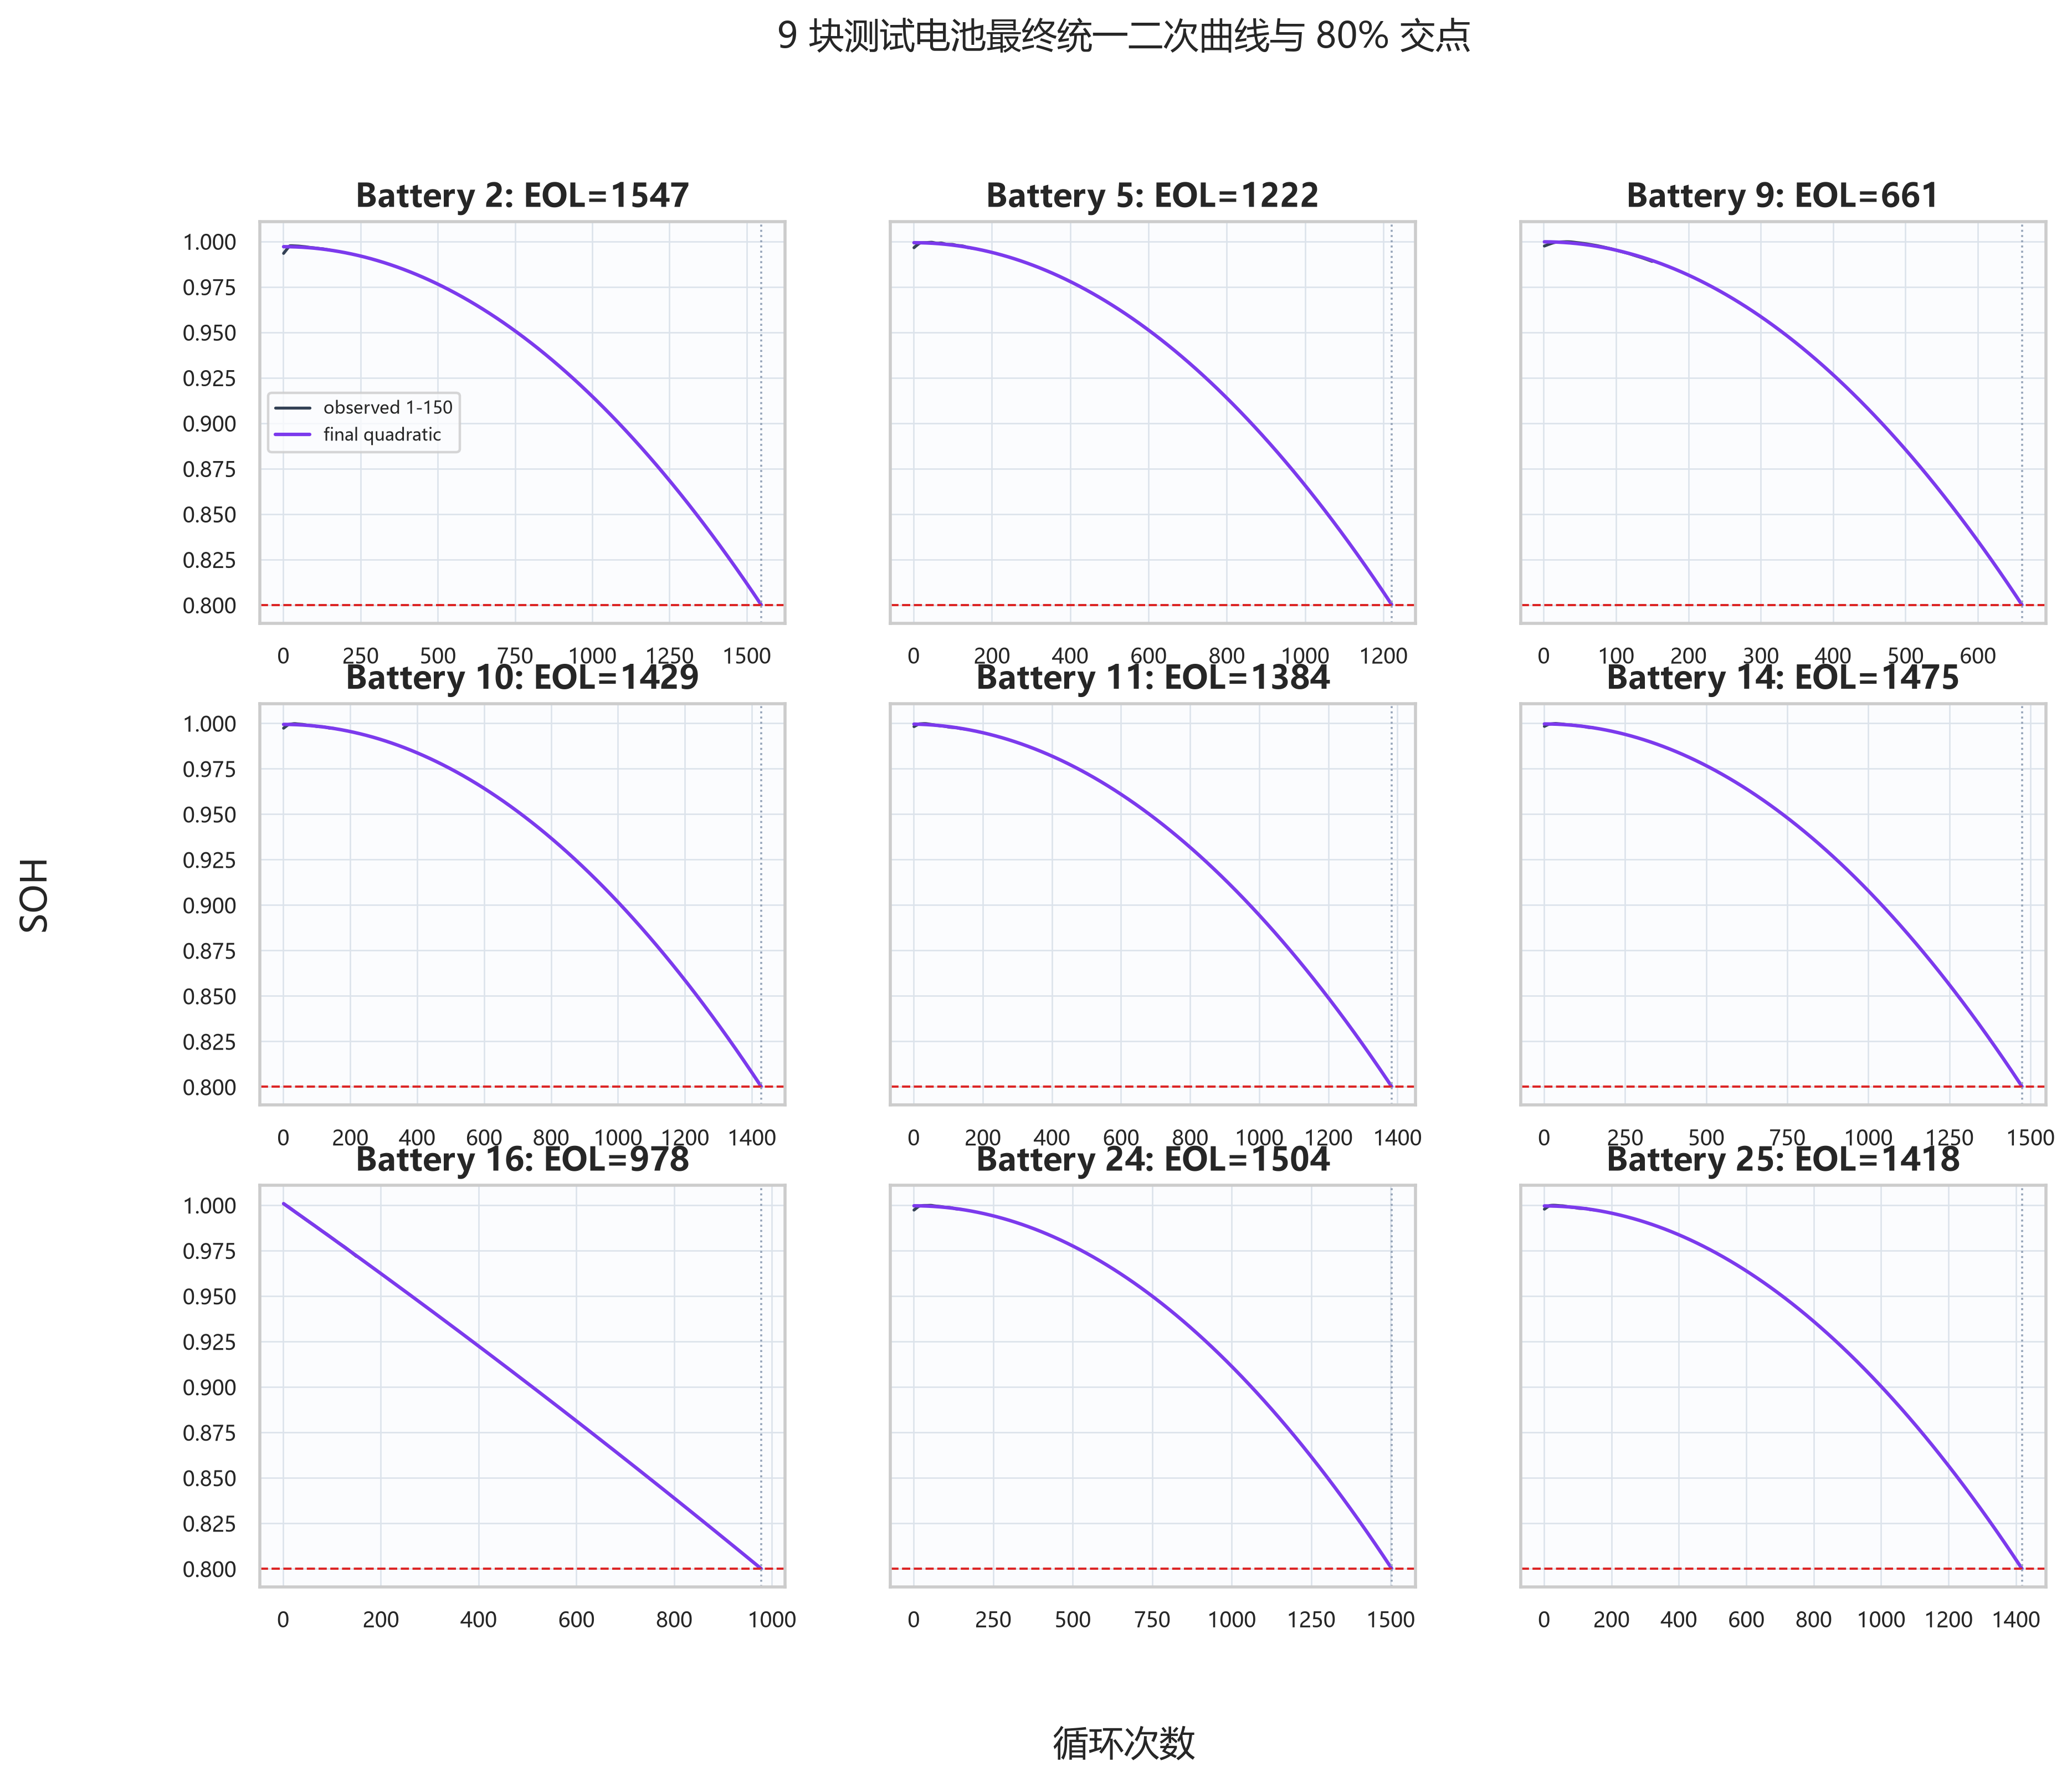
\includegraphics[width=0.96\textwidth]{q3_s02_test_final_quadratic_eol_panels.png}
\caption{9 块测试电池最终统一二次曲线及 SOH=0.8 交点}
\label{fig:test-eol}
\end{figure}

\section{问题四：基于二次寿命函数的多目标优化}

\subsection{充电时间与寿命代理}

两阶段理想充电时间为
\begin{equation}
 T_{\rm ideal}=60\left[\frac{Q_1/100}{C_1}
 +\frac{(80-Q_1)/100}{C_2}\right].
\end{equation}
比较纯物理、固定偏移、$Q_1$ 线性/二次修正和仿射模型。dataset 3 中纯物理模型 LOSO RMSE 最小为 0.429 min，但固定偏移模型仅高 2.4\%，且能修正系统偏差，按既定低复杂度规则选择 physical offset，RMSE 为 0.439 min。

寿命端不再拟合 stress 到 EOL，而是直接使用问题二选定的策略模型：
\[
 (C_1,Q_1,C_2)\to(\widehat\Rone,\widehat A)
 \to(\widehat d_1,\widehat d_2)
 \to \widehat{\SOH}(n)\to \widehat L.
\]
所有候选取 $a=1$。训练电池的 $a$ 分布只在次级 bootstrap 中抽样，以量化初始状态偏移对寿命的影响。

\subsection{可信域、分组 bootstrap 与双 Pareto}

在 dataset 3 的观测参数矩形内以 $0.05$ C、1\% SOC 网格搜索，再取观测凸包与最近邻信任域交集。每次 bootstrap 先有放回抽取策略，再在策略内抽电池，重新拟合参数桥接并计算每个候选的 $d_1,d_2,L$；正式运行 1000 次，得到 $L_{\rm median}$、$L_{10}$、$L_{90}$ 和 95\% 区间。分别求
\[
 \min T,\ \max L_{\rm median};\qquad
 \min T,\ \max L_{10}.
\]
图\ref{fig:pareto} 显示中位寿命前沿和保守 P10 前沿位置存在明显差距，但三个主代表点同时位于 P10 非支配集合，说明前沿方向大体一致、寿命绝对值不确定。

\begin{figure}[H]
\centering
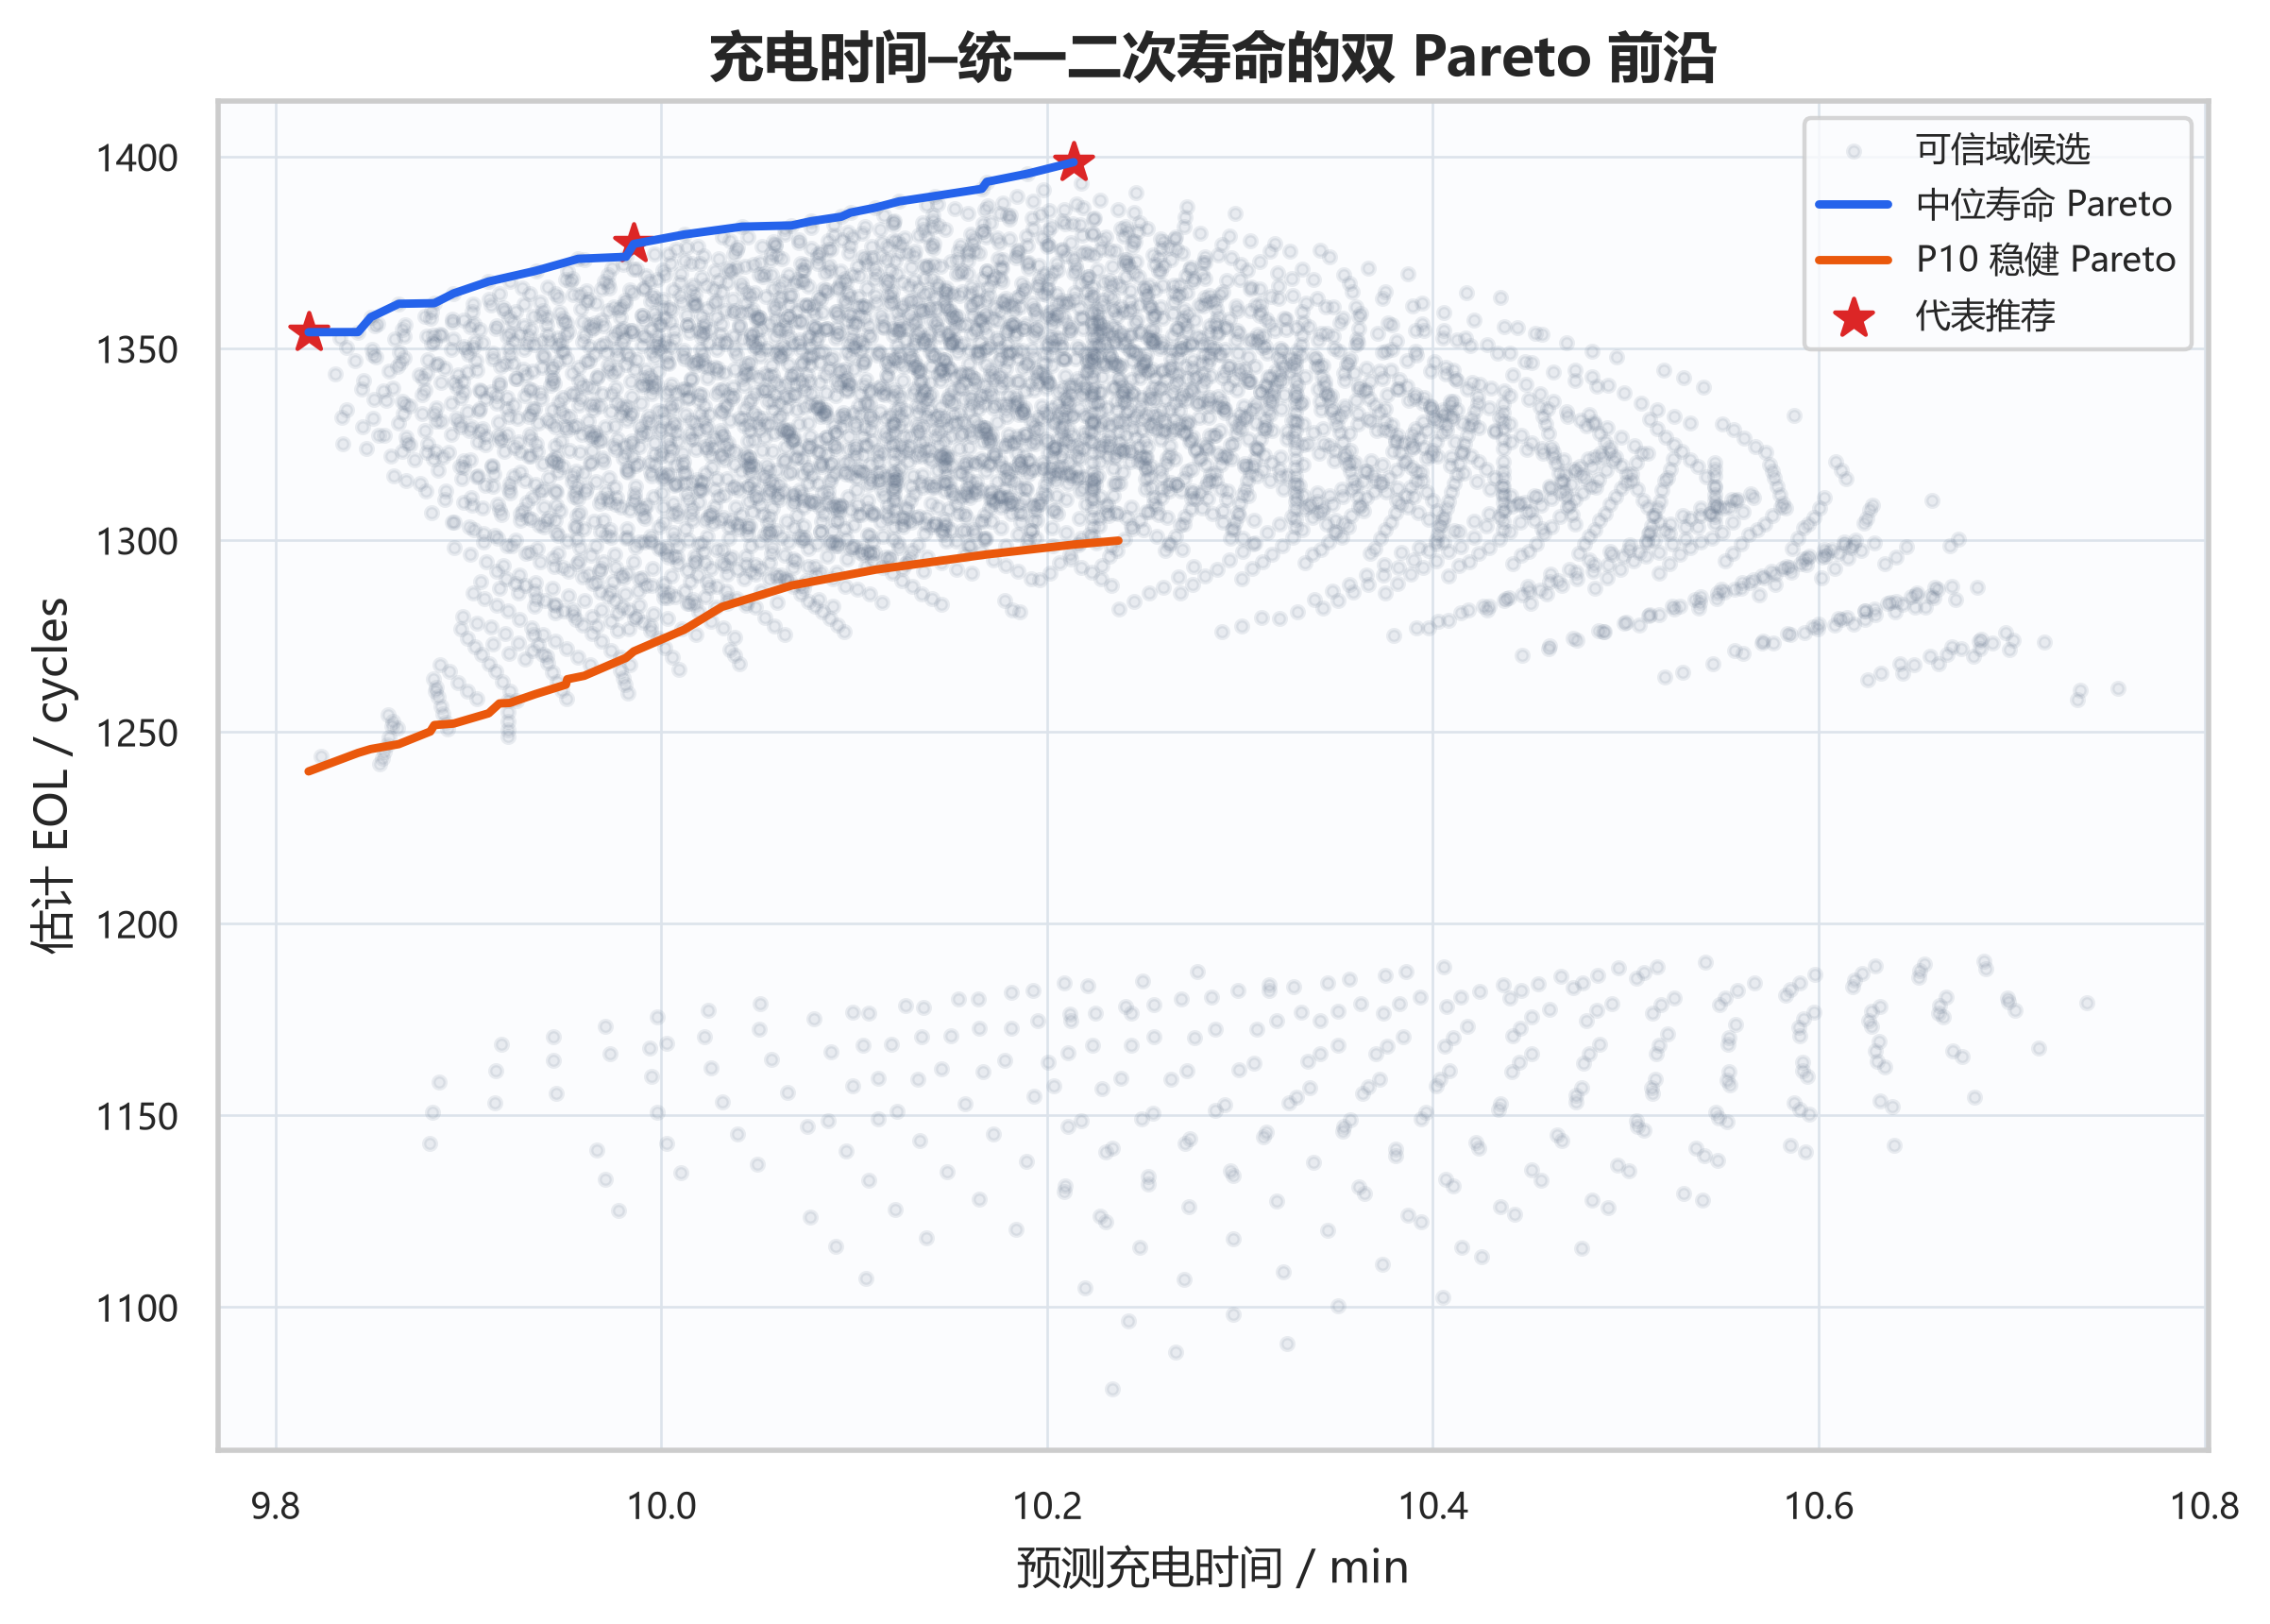
\includegraphics[width=0.82\textwidth]{q4_18_dual_pareto_fronts.png}
\caption{充电时间与统一二次寿命的中位/P10 双 Pareto 前沿}
\label{fig:pareto}
\end{figure}

\subsection{代表策略、边际收益与推荐等级}

快充点要求接近最短时间且不落入寿命极端区；寿命点在合理时间上限内最大化中位寿命；折中点最小化归一化目标到理想点的欧氏距离，明确称为 ideal-point compromise，而非未计算曲率的 knee。

\begin{table}[H]
\centering
\caption{统一二次模型的三类代表策略}
\begin{tabular}{lccccccc}
\toprule
类型 & $C_1$ & $Q_1$ & $C_2$ & $T$/min & SOH$_{200}$ & $L_{50}$ & $L_{10}$ \\
\midrule
快充优先 & 5.20 & 58 & 4.55 & 9.817 & 0.9919 & 1354 & 1240 \\
理想点折中 & 5.10 & 64 & 4.30 & 9.986 & 0.9930 & 1377 & 1271 \\
寿命优先 & 5.00 & 67 & 4.00 & 10.214 & 0.9941 & 1399 & 1299 \\
\bottomrule
\end{tabular}
\label{tab:recommendation}
\end{table}

从快充点移到折中点增加约 0.169 min，模型寿命中位数增加约 23 次；再增加 0.228 min 到寿命点，中位数再增加约 21 次。该收益小于 bootstrap 区间宽度，故应表述为“预测改善趋势”，不能表述为确定寿命提升。快充点 1000 次 bootstrap 的参数位置稳定；折中点落在主点一个缩放距离内的比例为 57.9\%，寿命点仅为 37.5\%，后两者应降级为推荐区域。

\begin{figure}[H]
\centering
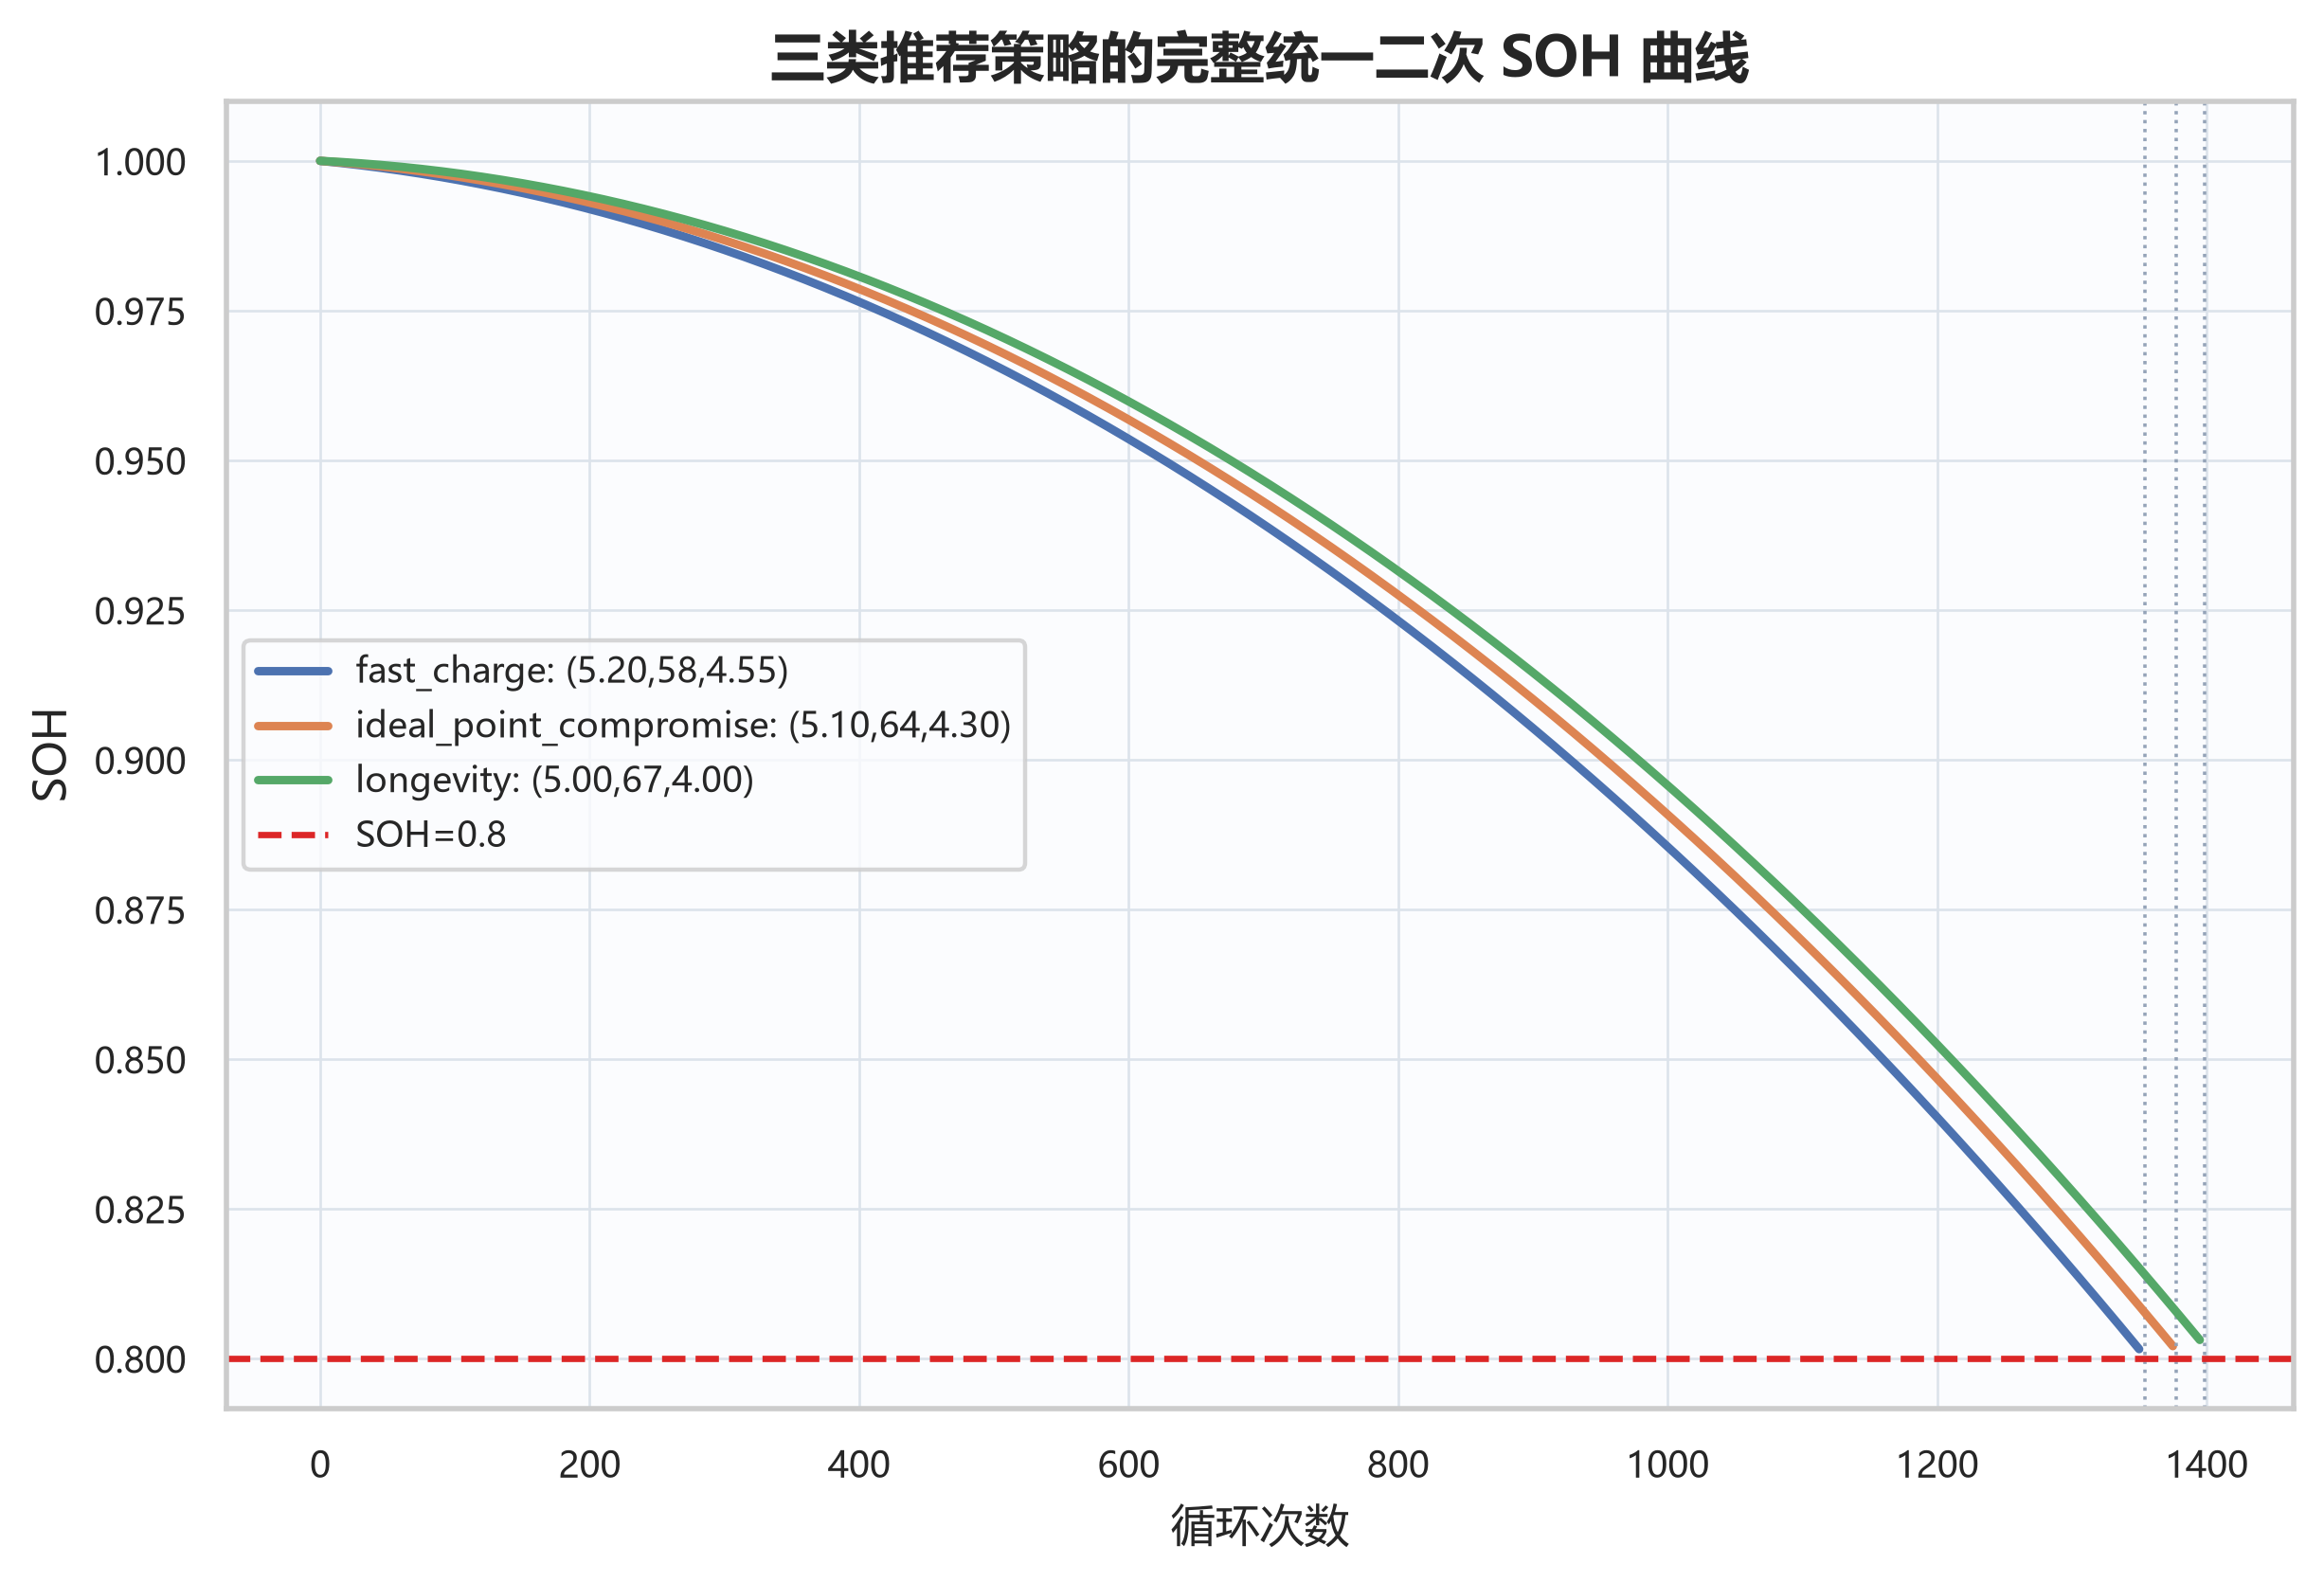
\includegraphics[width=0.82\textwidth]{q4_19_recommended_full_curves.png}
\caption{三类代表策略的完整统一二次 SOH 曲线}
\label{fig:full-curves}
\end{figure}

\subsection{旧 stress baseline 与新主模型}

旧模型的路径为“参数 $\to$ 求和 SOC stress $\to$ 退化/EOL”，新模型直接预测二次参数。就同一 $\Rone,A$ 响应而言，新原始参数桥接的综合 LOSO 1.142 优于求和 stress 的 1.229；但在旧定义下，SOC stress 对已观测策略 EOL 的重现 MAE 为 88 次，新 $a=1$ 二次桥接为 118 次，二者的 EOL 基准不同，不能据此作严格同尺度排名。图\ref{fig:oldnew} 显示旧前沿给出的寿命水平更低、区域也不同。

新模型的优势是从问题一到四共享同一可解释寿命函数并能传播 $d_1,d_2$ 不确定性；代价是只有 6 个独立策略点，LOSO 和推荐区域都不稳定。故本文选择新模型作为主论述，但不隐瞒旧 stress 在局部经验拟合上的优势。

\begin{figure}[H]
\centering
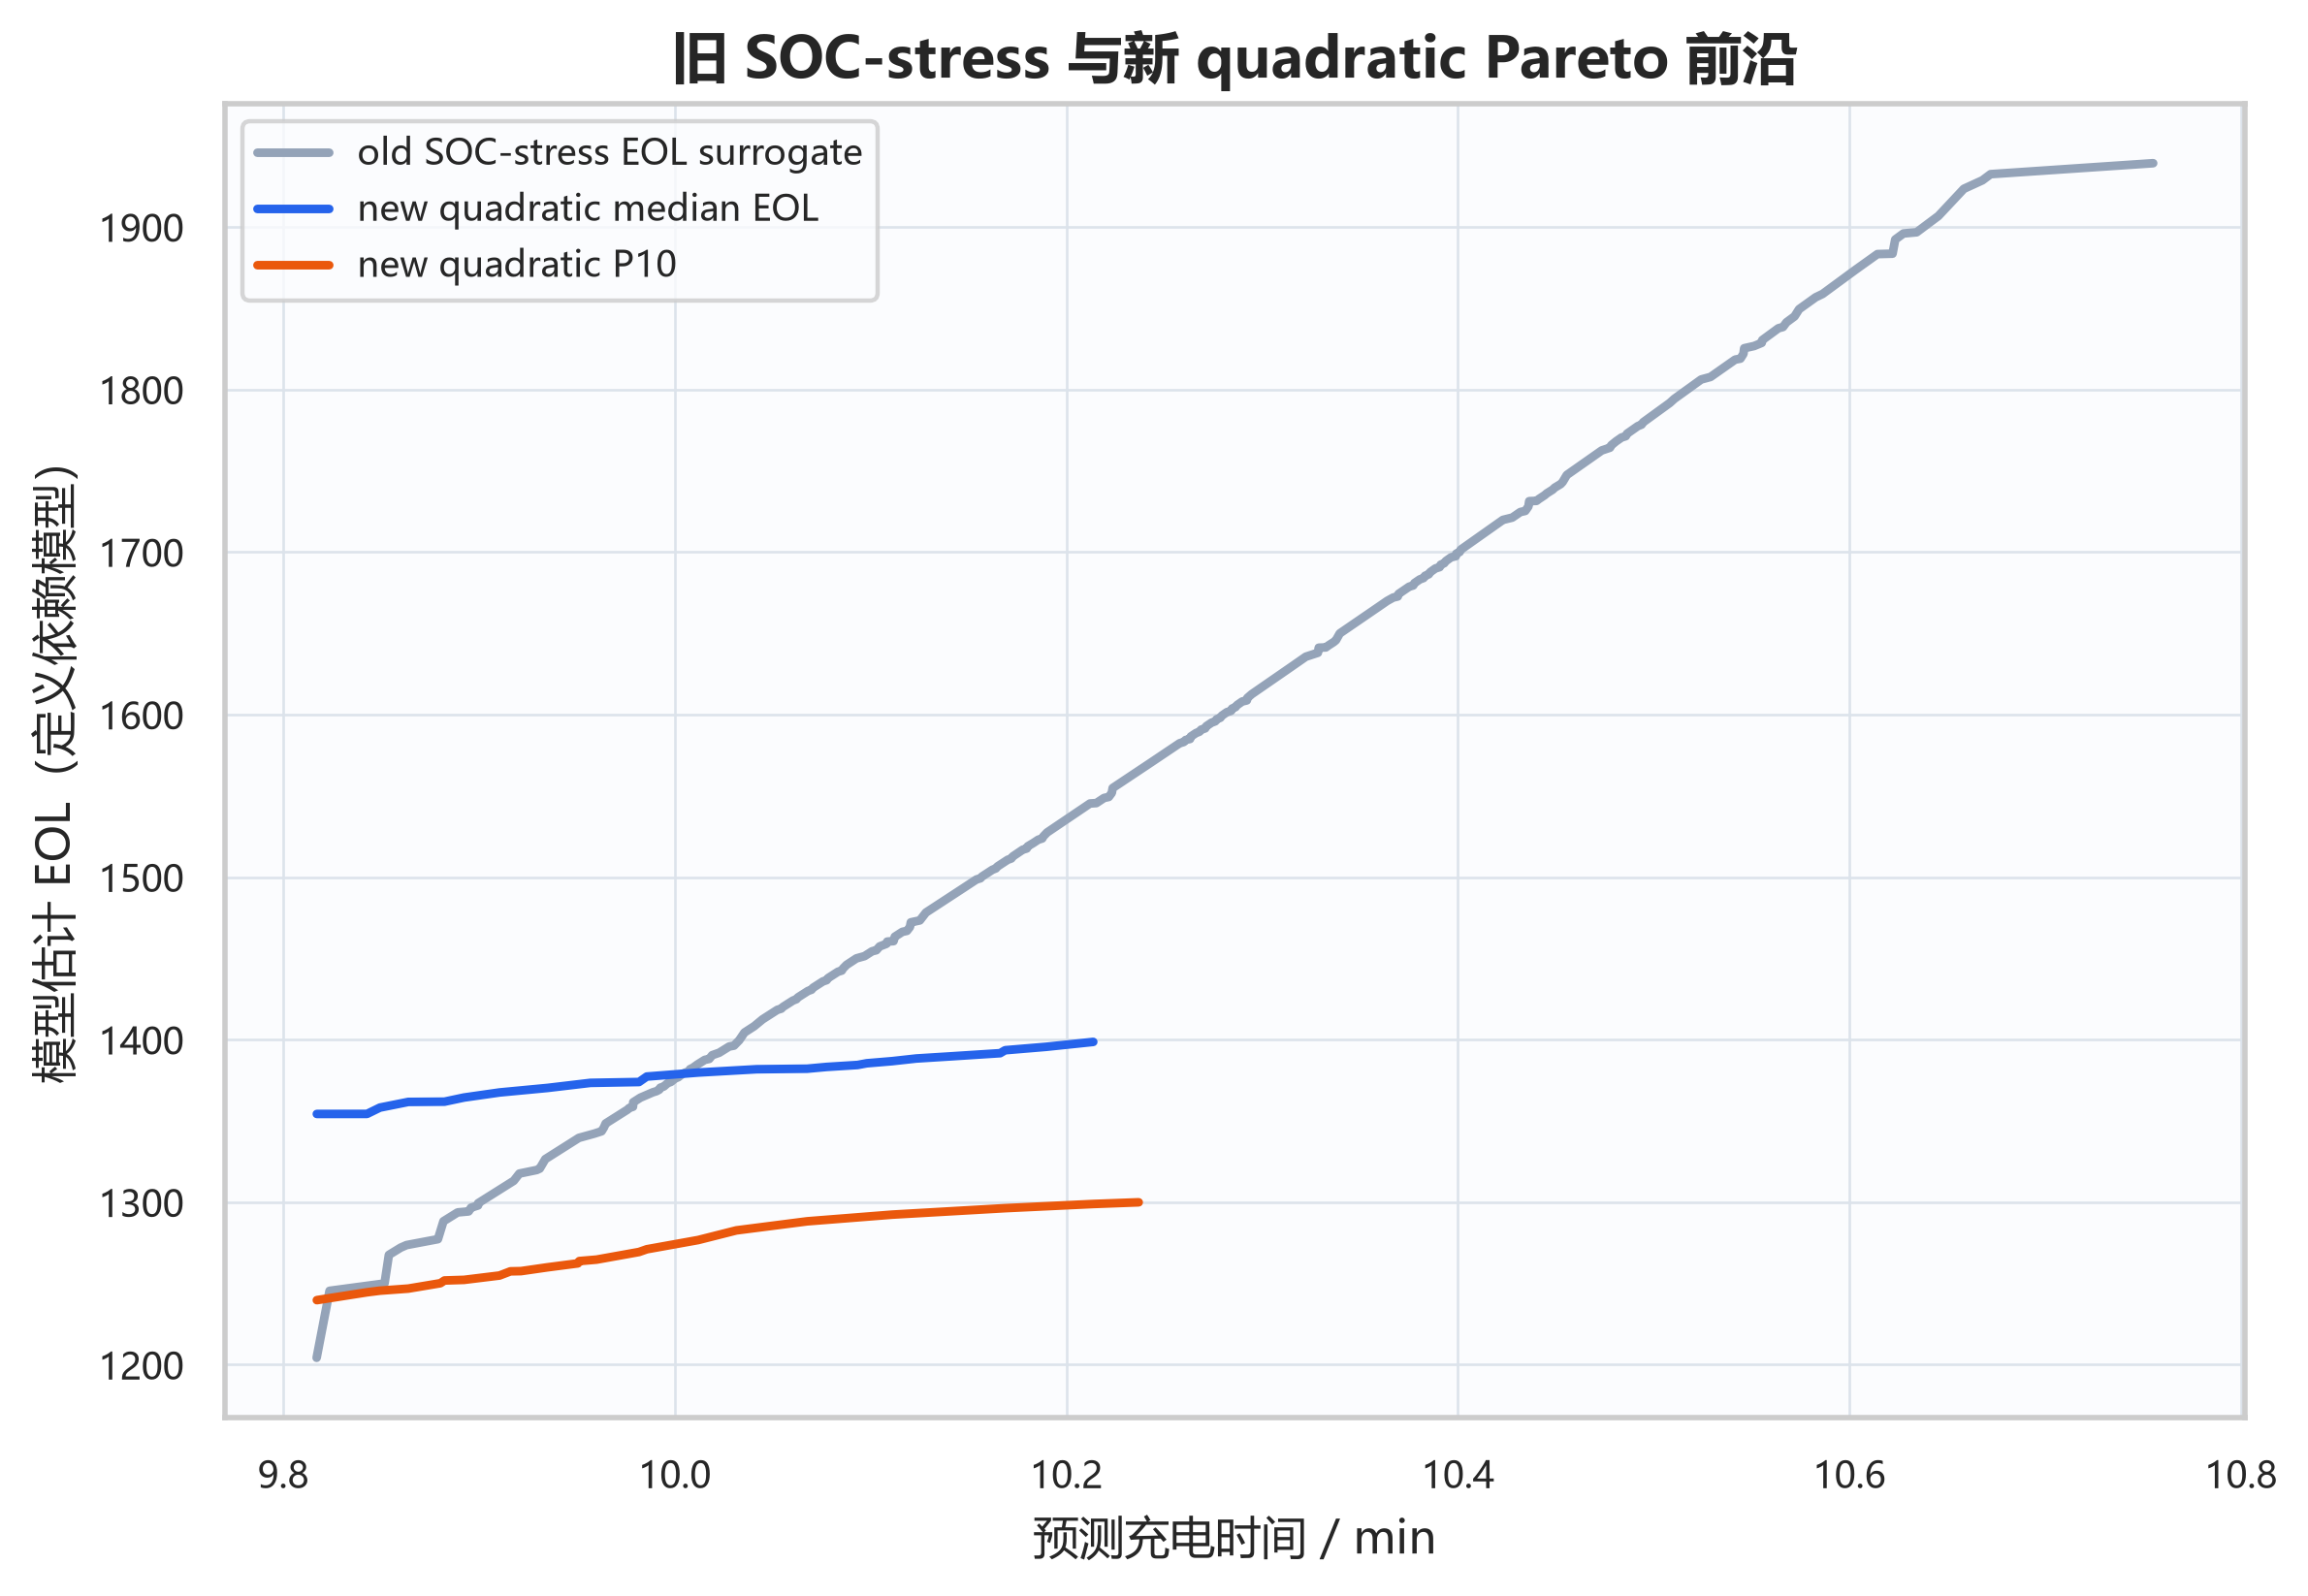
\includegraphics[width=0.80\textwidth]{q4_s01_old_stress_vs_new_quadratic_pareto.png}
\caption{旧 SOC stress 与新统一 quadratic 的 Pareto 对照}
\label{fig:oldnew}
\end{figure}

\section{敏感性、局限与可靠性分层}

\subsection{敏感性分析}

完成以下检查：$p=1,1.5,2,2.5,3$ 的两阶段暴露；矩形、凸包、最近邻信任域及其交集；逐一删除 dataset 3 策略；全参数化数据与 dataset 3；训练电池 $a$ 分布；1000 次分组 bootstrap。不同 $p$ 的 LOSO 均接近且普遍大于 1，禁止把某个指数解释为物理定律。可信域放宽时折中与寿命点会漂移；逐策略删除也会显著改变参数桥接，说明当前适合报告区域而非小数点后精确方案。

\subsection{结论可靠性}

\begin{table}[H]
\centering
\caption{结论的可靠性分层}
\begin{tabularx}{0.94\textwidth}{p{3.0cm}p{2.3cm}X}
\toprule
结论 & 等级 & 依据与限制 \\
\midrule
151--200 次短期预测 & 较高 & 40 块训练电池有真实未来，可严格时间顺序验证 \\
quadratic 作为统一函数 & 条件稳健 & 单调、低参数且截断表现可接受；长期 EOL 仍结构敏感 \\
$d_1,d_2$ 个体分解 & 有限 & 37.5\% 命中边界，bootstrap 补偿显著 \\
$Q_1/C_2$ 参数方向 & 趋势性 & 某些系数方向稳定，但 LOSO 未优于均值且受 batch 混杂 \\
早期 IR/T 机制关联 & 不支持 & 整策略留出时 M2 无稳定增益 \\
测试电池 EOL & 中低 & 无真实 EOL，只能用 bootstrap 与截断变化评价 \\
Pareto 推荐 & 中低 & 处于可信域但仅 6 个策略点，未经新实验验证 \\
\bottomrule
\end{tabularx}
\end{table}

\section{结论与建议}

本文没有为四问分别发明寿命指标，而是固定
\[
  \SOH(n)=a-d_1n/100-d_2(n/100)^2
\]
作为唯一最终寿命函数。问题一发现原生 $d_1,d_2$ 在个体 bootstrap 中存在强补偿，策略级改用 $\Rone,A$ 建模；问题二表明稀疏设计只能支持少量方向性关联，不能声称独立因果参数效应；问题三证明策略先验当前未改善 151--200 次预测，因此短期采用验证更优的 ensemble，再回归统一二次曲线求寿命；问题四把参数桥接直接传播到完整 SOH 和 EOL，在严格可信域中给出快充、折中与寿命三类候选。

若开展后续实验，优先在 $(C_1,Q_1,C_2)\approx(5.0\!\sim\!5.2,58\!\sim\!67,4.0\!\sim\!4.55)$ 的推荐区域补充正交或近正交设计，并增加每策略电池数。新实验应覆盖 EOL 或至少显著超过 200 次，以检验 $d_2$ 的长期可辨识性；同时固定结构与批次，避免再把结构差异误归因于充电参数。只有经这些实验确认后，模型推荐才能升级为工程结论。

\begin{thebibliography}{99}
\bibitem{severson2019} Severson K A, Attia P M, Jin N, et al. Data-driven prediction of battery cycle life before capacity degradation[J]. Nature Energy, 2019, 4: 383--391.
\bibitem{attia2020} Attia P M, Grover A, Jin N, et al. Closed-loop optimization of fast-charging protocols for batteries with machine learning[J]. Nature, 2020, 578: 397--402.
\bibitem{lowess} Cleveland W S. Robust locally weighted regression and smoothing scatterplots[J]. Journal of the American Statistical Association, 1979, 74(368): 829--836.
\bibitem{theilsen} Sen P K. Estimates of the regression coefficient based on Kendall's tau[J]. Journal of the American Statistical Association, 1968, 63(324): 1379--1389.
\bibitem{ridge} Hoerl A E, Kennard R W. Ridge regression: biased estimation for nonorthogonal problems[J]. Technometrics, 1970, 12(1): 55--67.
\bibitem{bootstrap} Efron B, Tibshirani R J. An Introduction to the Bootstrap[M]. New York: Chapman and Hall, 1993.
\end{thebibliography}

\appendix
\section{结果文件与复现说明}

旧问题一至四的结果保留在原问题目录；本次统一重构写入独立目录：
\begin{itemize}
  \item baseline：\path{outputs/question1--4}，\path{figures/question1--4}；
  \item unified：\path{outputs/unified_quadratic_v2}，\path{figures/unified_quadratic_v2}。
\end{itemize}
正式运行命令为：
\begin{lstlisting}[language={}]
.\.venv\Scripts\python.exe scripts\run_unified_refactor.py
.\.venv\Scripts\python.exe -m pytest -q
\end{lstlisting}
正式参数包括：单电池 bootstrap 300 次，策略系数 bootstrap 1000 次，问题四候选寿命 bootstrap 1000 次，测试电池 EOL bootstrap 300 次。全部随机过程固定种子 20260815。

\section{关键输出表}

问题一表包括每电池二次参数、边界、bootstrap、100/150/200 截断稳定性；问题二表包括策略级中位数、OLS/Ridge、LOSO、VIF、两阶段暴露、局部匹配、早期健康 LOBO 和七通道证据矩阵；问题三表包括全部伪测试逐循环预测、误差、区间、消融、测试电池预测及 EOL；问题四表包括充电时间验证、完整可信域候选、中位/P10 Pareto、三类推荐、逐策略删除、$p$ 敏感性和旧新模型比较。

\section{AI 工具使用说明}

分析代码、表格和论文排版在 AI 编程工具辅助下完成；模型假设、数据边界、交叉验证规则与结论强度均由作者审阅。未调用外部完整寿命数据库，未利用 global id 查询真实 EOL，也未将测试电池未知未来用于训练。所有可复现代码和结果表随支撑材料提交。

\end{document}
